\section{Pendahuluan}
\subsection{Latar Belakang}
Pada modul ini, kita akan membahas konfigurasi routing static dan routing dinamis pada perangkat
MikroTik. Routing merupakan proses pengiriman data antara dua atau lebih jaringan yang berbeda.
Dalam modul ini, kita akan membahas konsep dasar routing, macam-macam routing statis dan
dinamis, serta langkah-langkah untuk mengkonfigurasi kedua jenis routing ini pada perangkat
MikroTik.\\\\
Sebelum memulai pembahasan routing, penting untuk memahami konsep dasar jaringan dan
subnetting. Jaringan terdiri dari sejumlah perangkat yang terhubung satu sama lain, seperti komputer,
printer, dan perangkat jaringan lainnya. Setiap perangkat dalam jaringan memiliki alamat IP yang
unik.\\\\
Subnetting adalah proses pembagian jaringan menjadi subnet yang lebih kecil. Dengan subnetting, kita
dapat mengoptimalkan penggunaan alamat IP dan membagi jaringan menjadi beberapa segmen yang
terpisah.\\\\
Dalam routing, terdapat yang namanya protokol routing. Protokol routing adalah aturan yang
digunakan oleh perangkat jaringan untuk memilih jalur terbaik bagi pengiriman data antara jaringan
yang berbeda. Ada dua jenis protokol routing utama: \textbf{routing static dan routing dinamis.}

\subsection{Maksud dan Tujuan}
Mengetahui dan memahami konfigurasi routing static dan routing dinamis pada Mikrotik.

\subsection{Hasil yang diharapkan}
Dapat mengkonfigurasi konfigurasi routing static dan routing dinamis pada Mikrotik dengan
tepat.

%===========================================================%
\section{Tugas Pendahuluan}


\begin{center}
	\colorbox{cyan!30}{\parbox{0.8\linewidth}{
		\begin{enumerate}
		\item Buatlah topologi jaringan percobaan 1, 2, dan 3!
		\item Perbedaan Static Routing dan Dynamic Routing.
		\item Keuntungan dan kekurangan Static Routing dan Dynamic Routing
	\end{enumerate}
	}}
\end{center}

%===========================================================%
\section{Alat dan Bahan}
\begin{itemize}[label=$\bullet$, itemsep=-1pt, leftmargin=*]
	\item 2 perangkat router mikrotik.
	\item Aplikasi Winbox.
	\item 3 kabel LAN
\end{itemize}

%===========================================================%
\section{Jangka Waktu Pelaksanaan}
Pemahaman dan konfigurasi 1 jam.

%===========================================================%
\section{Penjelasan dan Tahapan Konfigurasi}

%======================PERCOBAAN 1==========================%
\subsection{Routing Statis}
Pada routing statis, terdapat setidaknya 2 jenis, yaitu
\begin{enumerate}
	\item Default Route : digunakan ketika tidak ada rute spesifik yang cocok untuk tujuan pengiriman data. Jika tidak ada rute yang cocok, paket data akan dikirim melalui default route. Pada MikroTik, default route dinyatakan sebagai 0.0.0.0/0.
	\item Static Route : adalah jenis routing di mana administrator jaringan secara manual mengonfigurasi tabel routing pada setiap perangkat jaringan. Dalam routing static, rute yang ditentukan secara manual digunakan untuk mengarahkan paket data ke tujuan yang ditentukan.
\end{enumerate}

\begin{center}
	\textbf{Konfigurasi Router 1}
	\begin{enumerate}
		\item Buka aplikasi WinBox pada PC 1 dan lakukan koneksi ke Router 1. Neighbors > Refresh > Double click Router yang terdeteksi > Connect
		\begin{figure}[H]
			\centering
			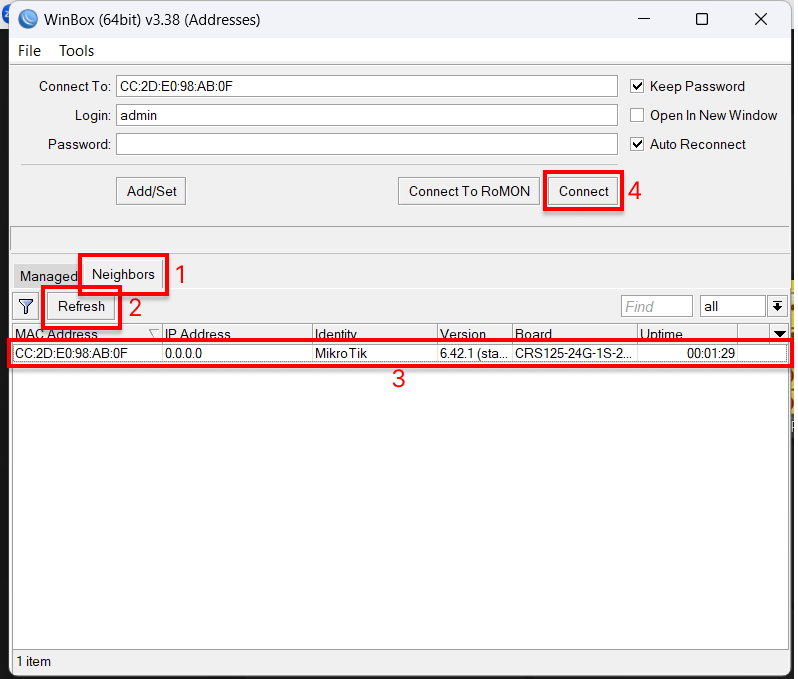
\includegraphics[width=0.8\linewidth]{P2/img/per1/pc1/Step 1.png}
			\caption{Step 1}
			\label{fig:Step 1(Per.1 PC1)}
		\end{figure}
		\item Berikan IP address pada interface ether2 dan ether 4 yang dapat dibuat pada tab IP > Addresses. Berikan IP address sesuai dengan cara pengaturan IP address yang benar. Berikan IP address yang berbeda dengan contoh di modul.
		\begin{figure}[H]
			\centering
			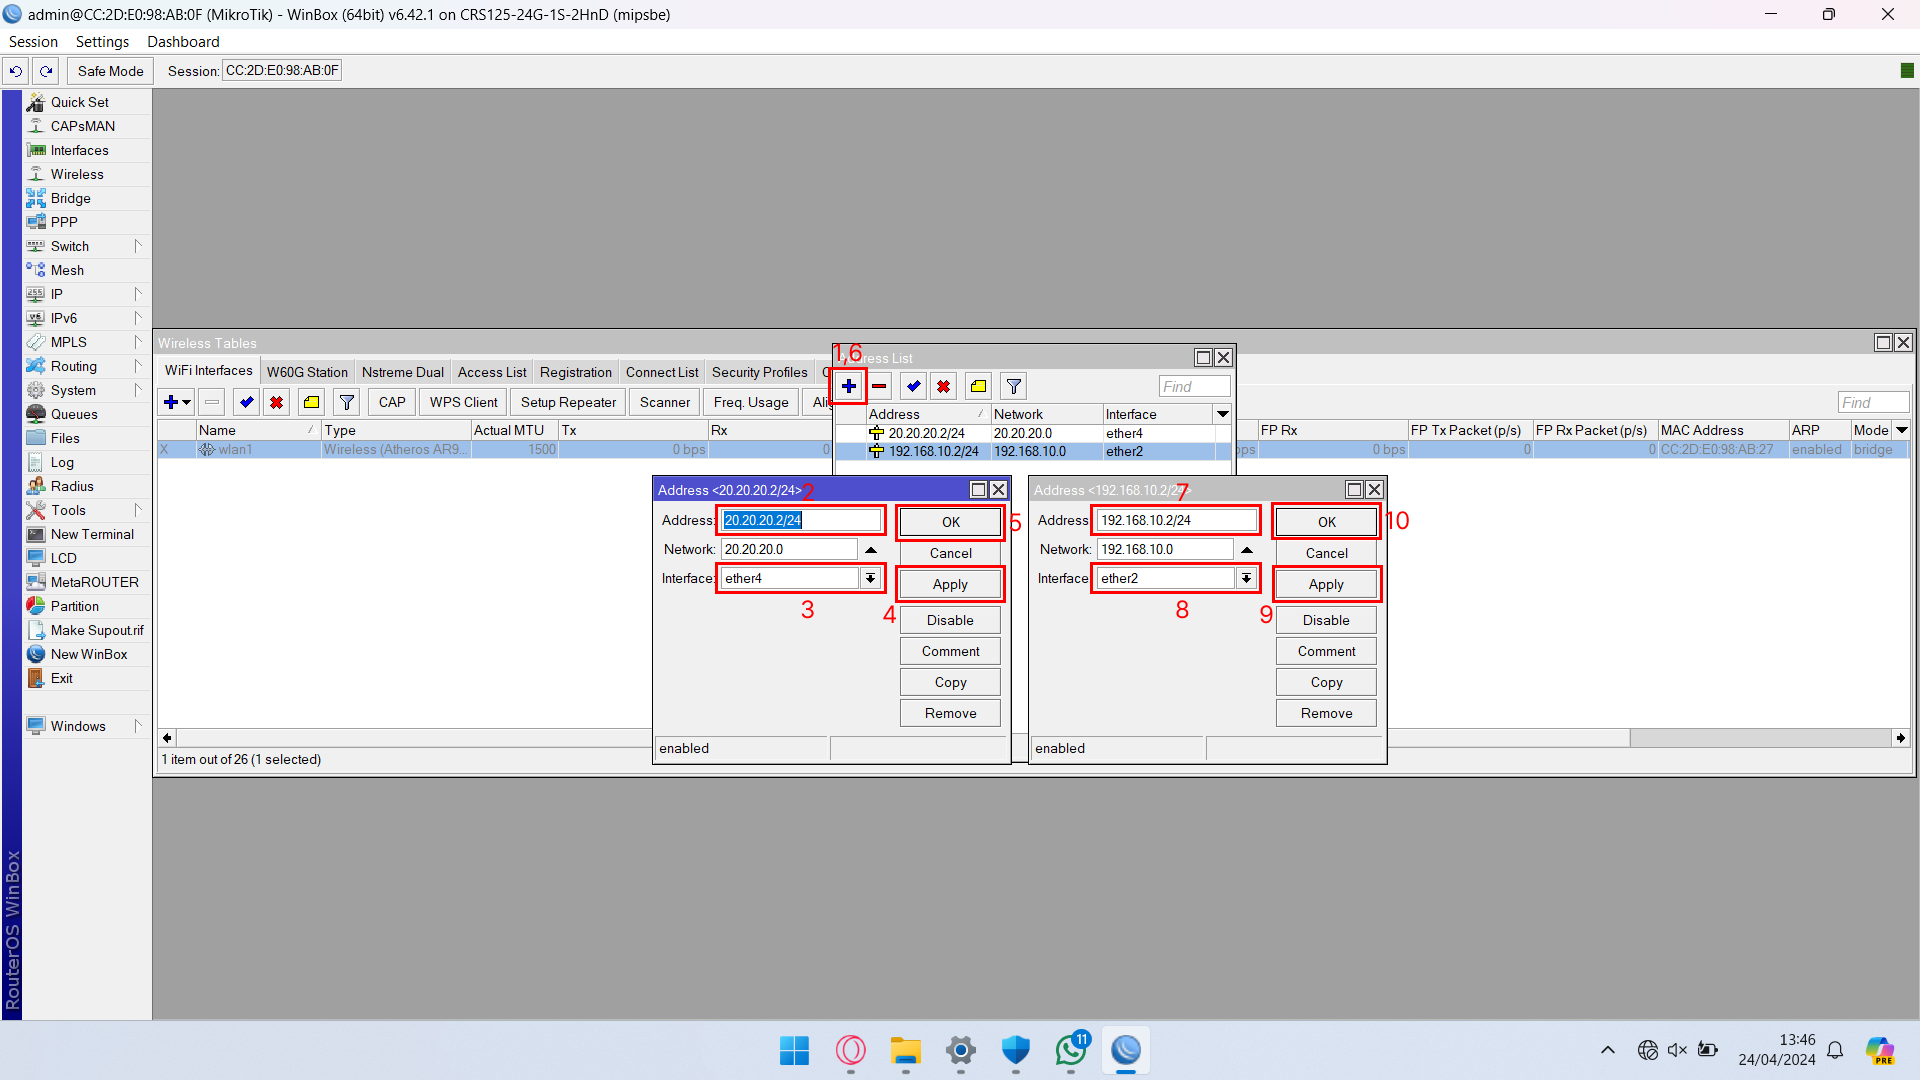
\includegraphics[width=0.9\linewidth]{P2/img/per1/pc1/Step 2.png}
			\caption{Step 2}
			\label{fig:Step 2(Per.1 PC1)}
		\end{figure}
		\item Lakukan routing statis. Buka pada tab IP > Routes, lalu tambahkan jaringan. 
		\begin{figure}[H]
			\centering
			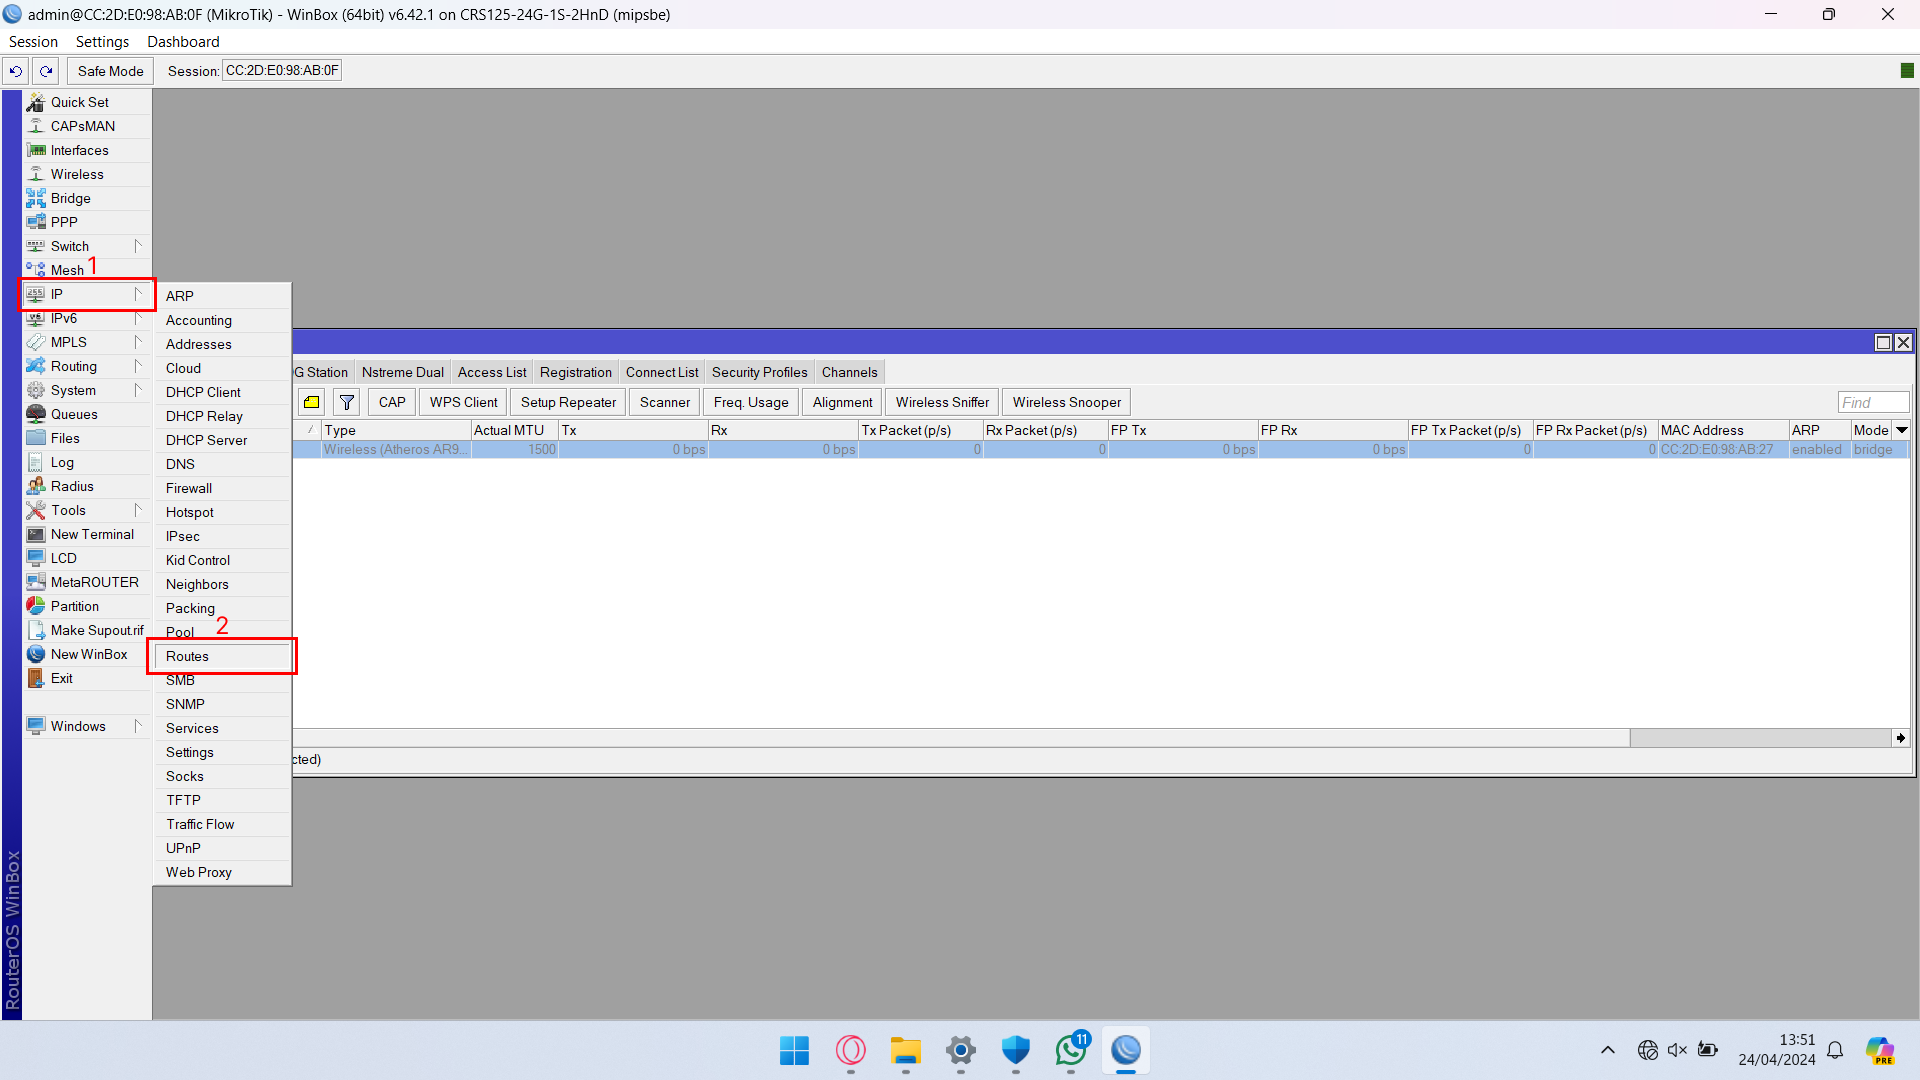
\includegraphics[width=0.9\linewidth]{P2/img/per1/pc1/Step 3.1.png}
			\caption{Step 3.1}
			\label{fig:Step 3.1(Per.1 PC1)}
		\end{figure}
		Masukkan alamat jaringan yang ingin dituju, melalui alamat Gateway pada router 2
		\begin{figure}[H]
			\centering
			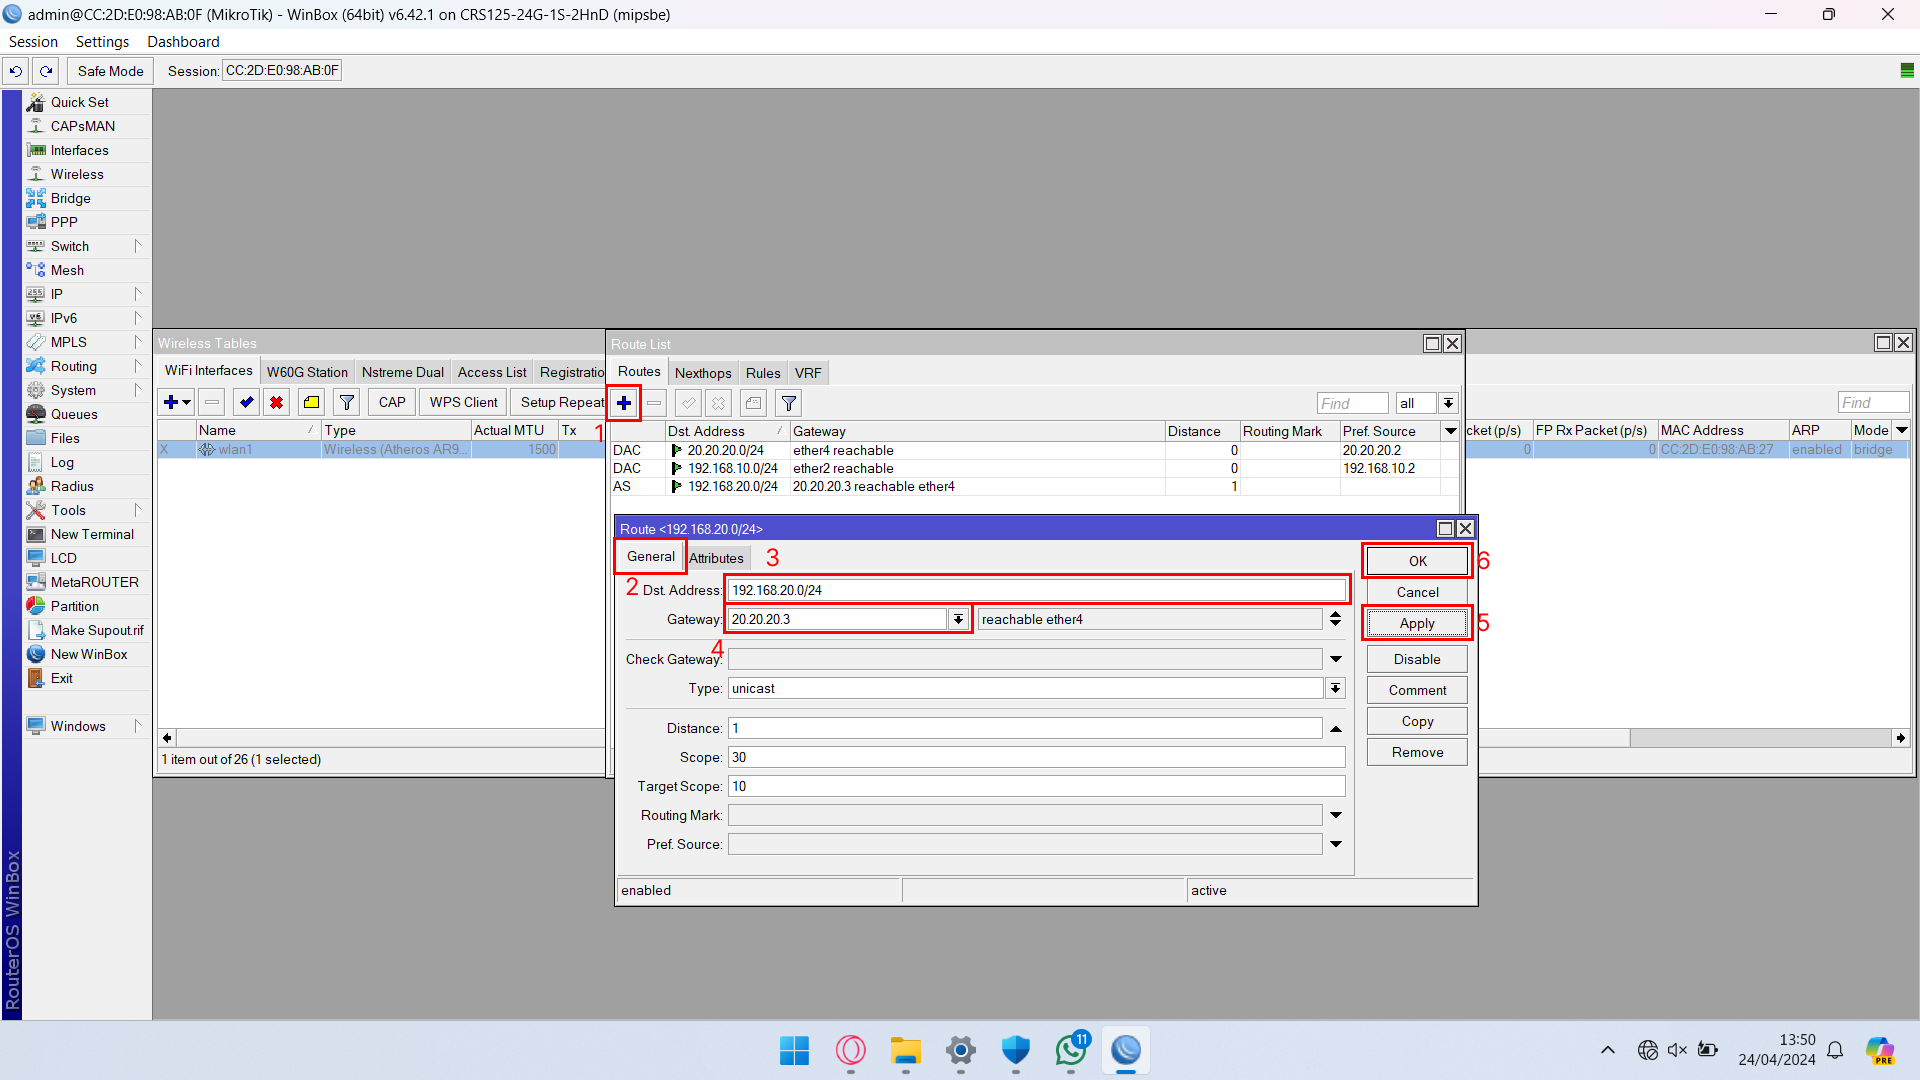
\includegraphics[width=0.9\linewidth]{P2/img/per1/pc1/Step 3.2.png}
			\caption{Step 3.2}
			\label{fig:Step 3.2(Per.1 PC1)}
		\end{figure}
	\end{enumerate}

	\textbf{Konfigurasi Router 2}
	\begin{enumerate}
		\item Buka WinBox dan lakukan koneksi ke Router 2
		\item Berikan IP address pada interface ether2 dan ether 4 yang dapat dibuat pada tab IP > Addresses. Berikan IP address sesuai dengan cara pengaturan IP address yang benar. Berikan IP address yang berbeda dengan contoh di modul.
		\begin{figure}[H]
			\centering
			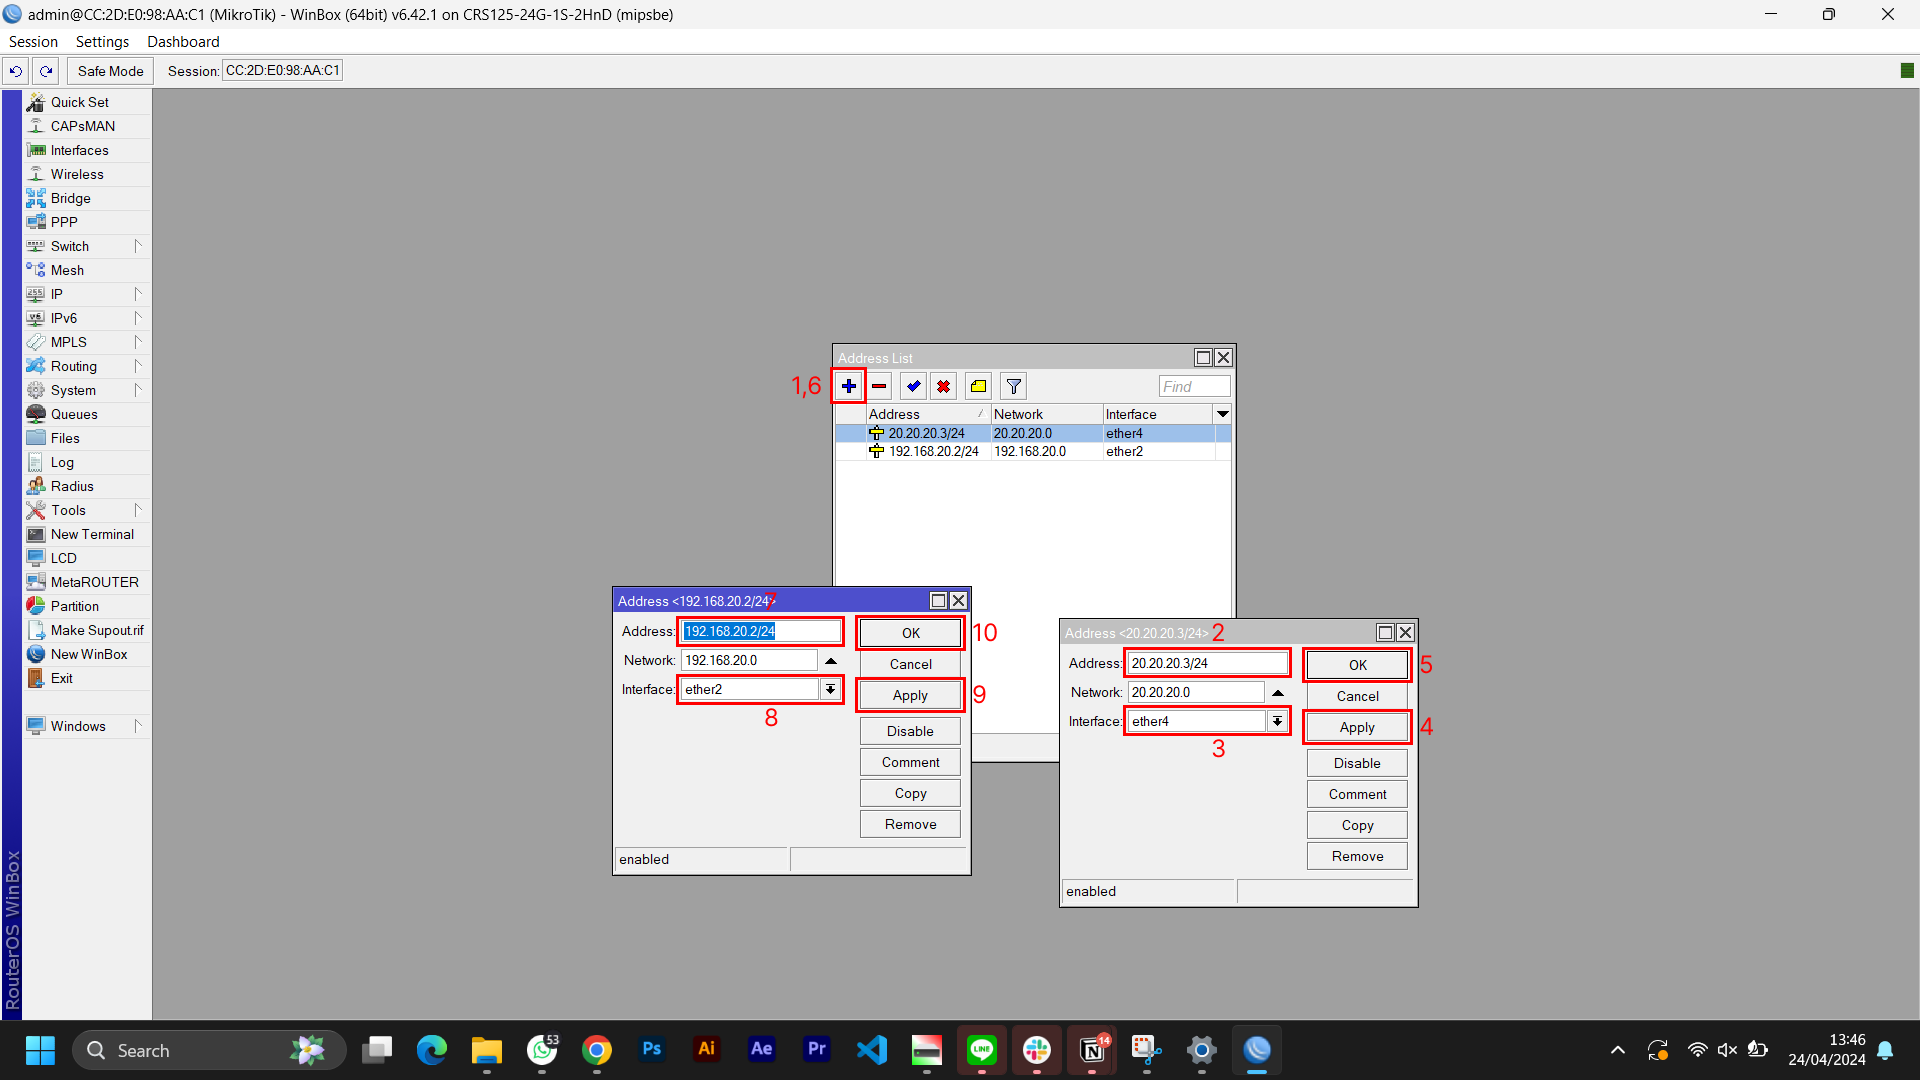
\includegraphics[width=0.9\linewidth]{P2/img/per1/pc2/Step 2.png}
			\caption{Step 2}
			\label{fig:Step 2(Per.1 PC2)}
		\end{figure}
		\item Lakukan routing statis. Buka pada tab IP > Routes, lalu tambahkan jaringan. Masukkan alamat jaringan yang ingin dituju, melalui alamat Gateway pada router 1
		\begin{figure}[H]
			\centering
			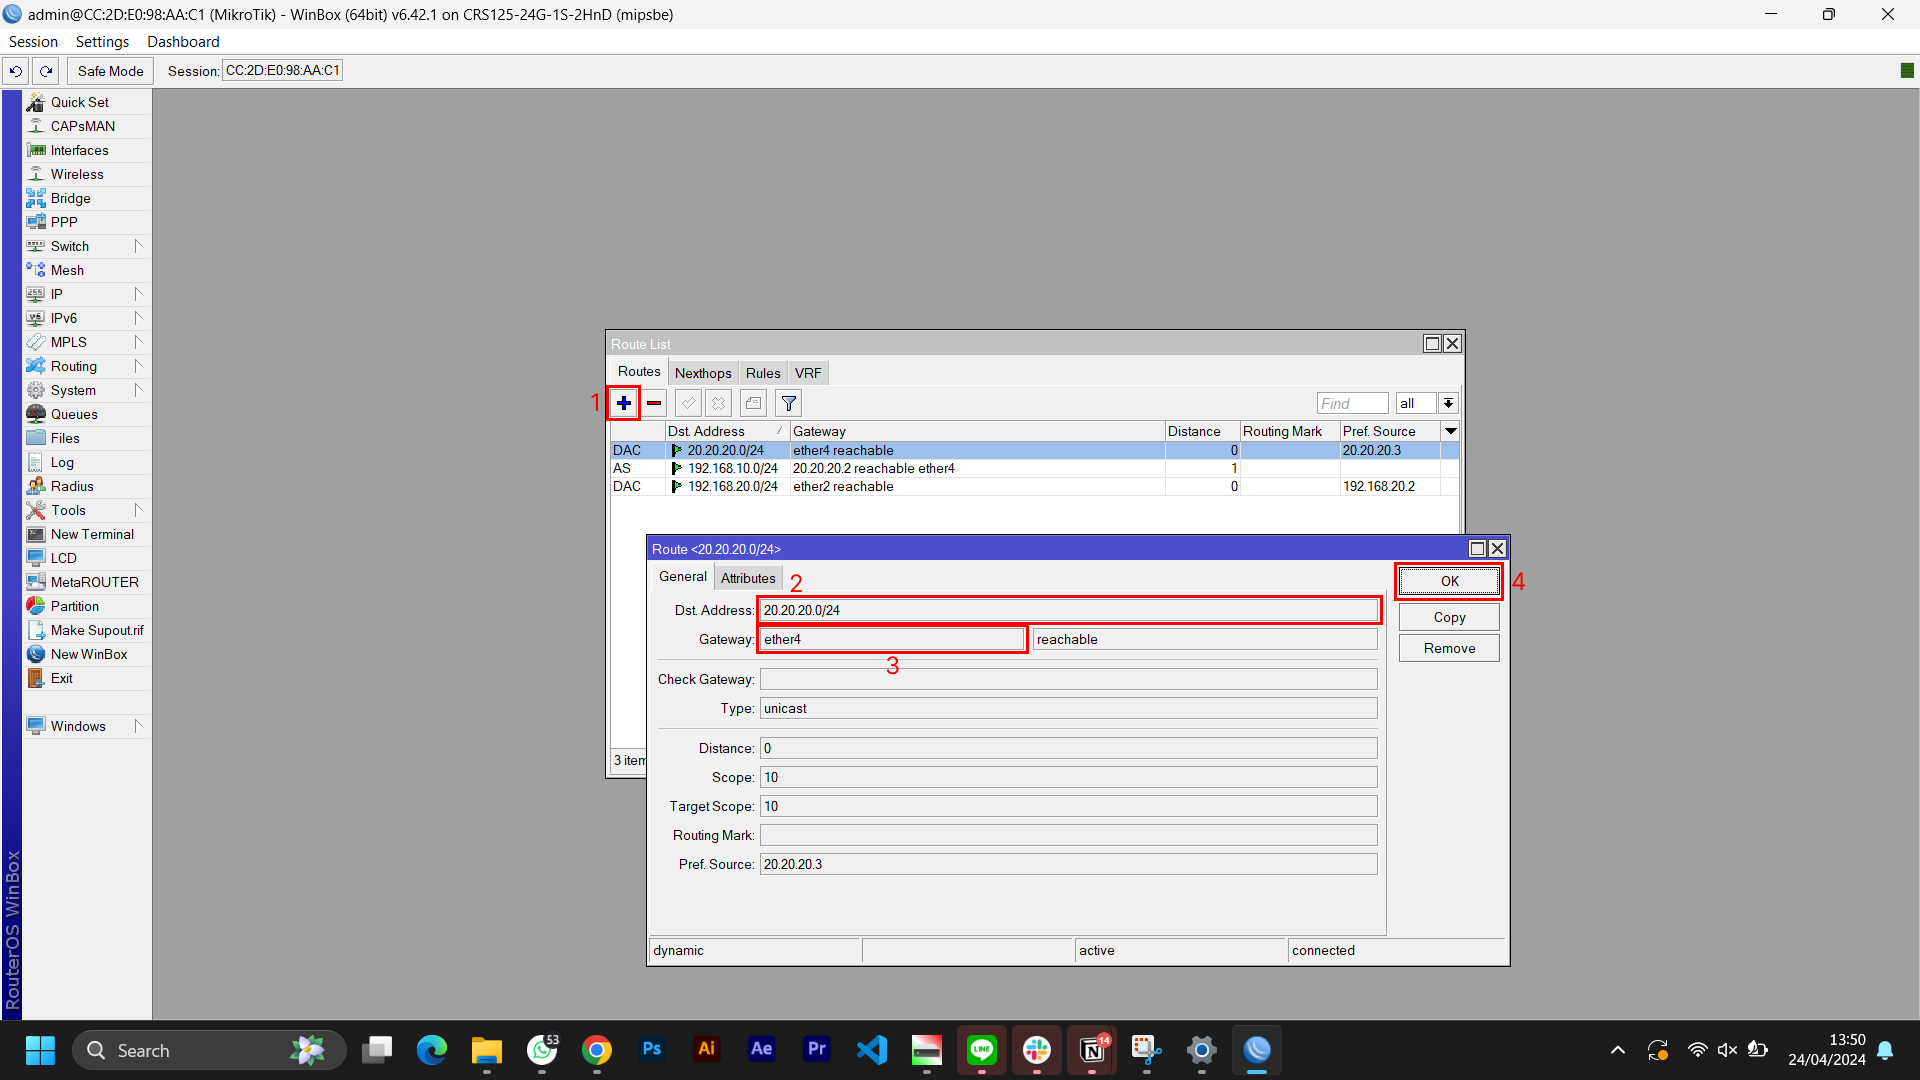
\includegraphics[width=0.9\linewidth]{P2/img/per1/pc2/Step 3.png}
			\caption{Step 3}
			\label{fig:Step 3(Per.1 PC2)}
		\end{figure}
	\end{enumerate}

	\textbf{Pengujian konfigurasi}
	\begin{enumerate}
		\item Lakukan tes ping ke Router 2 melalui Router 1
		\begin{figure}[H]
			\centering
			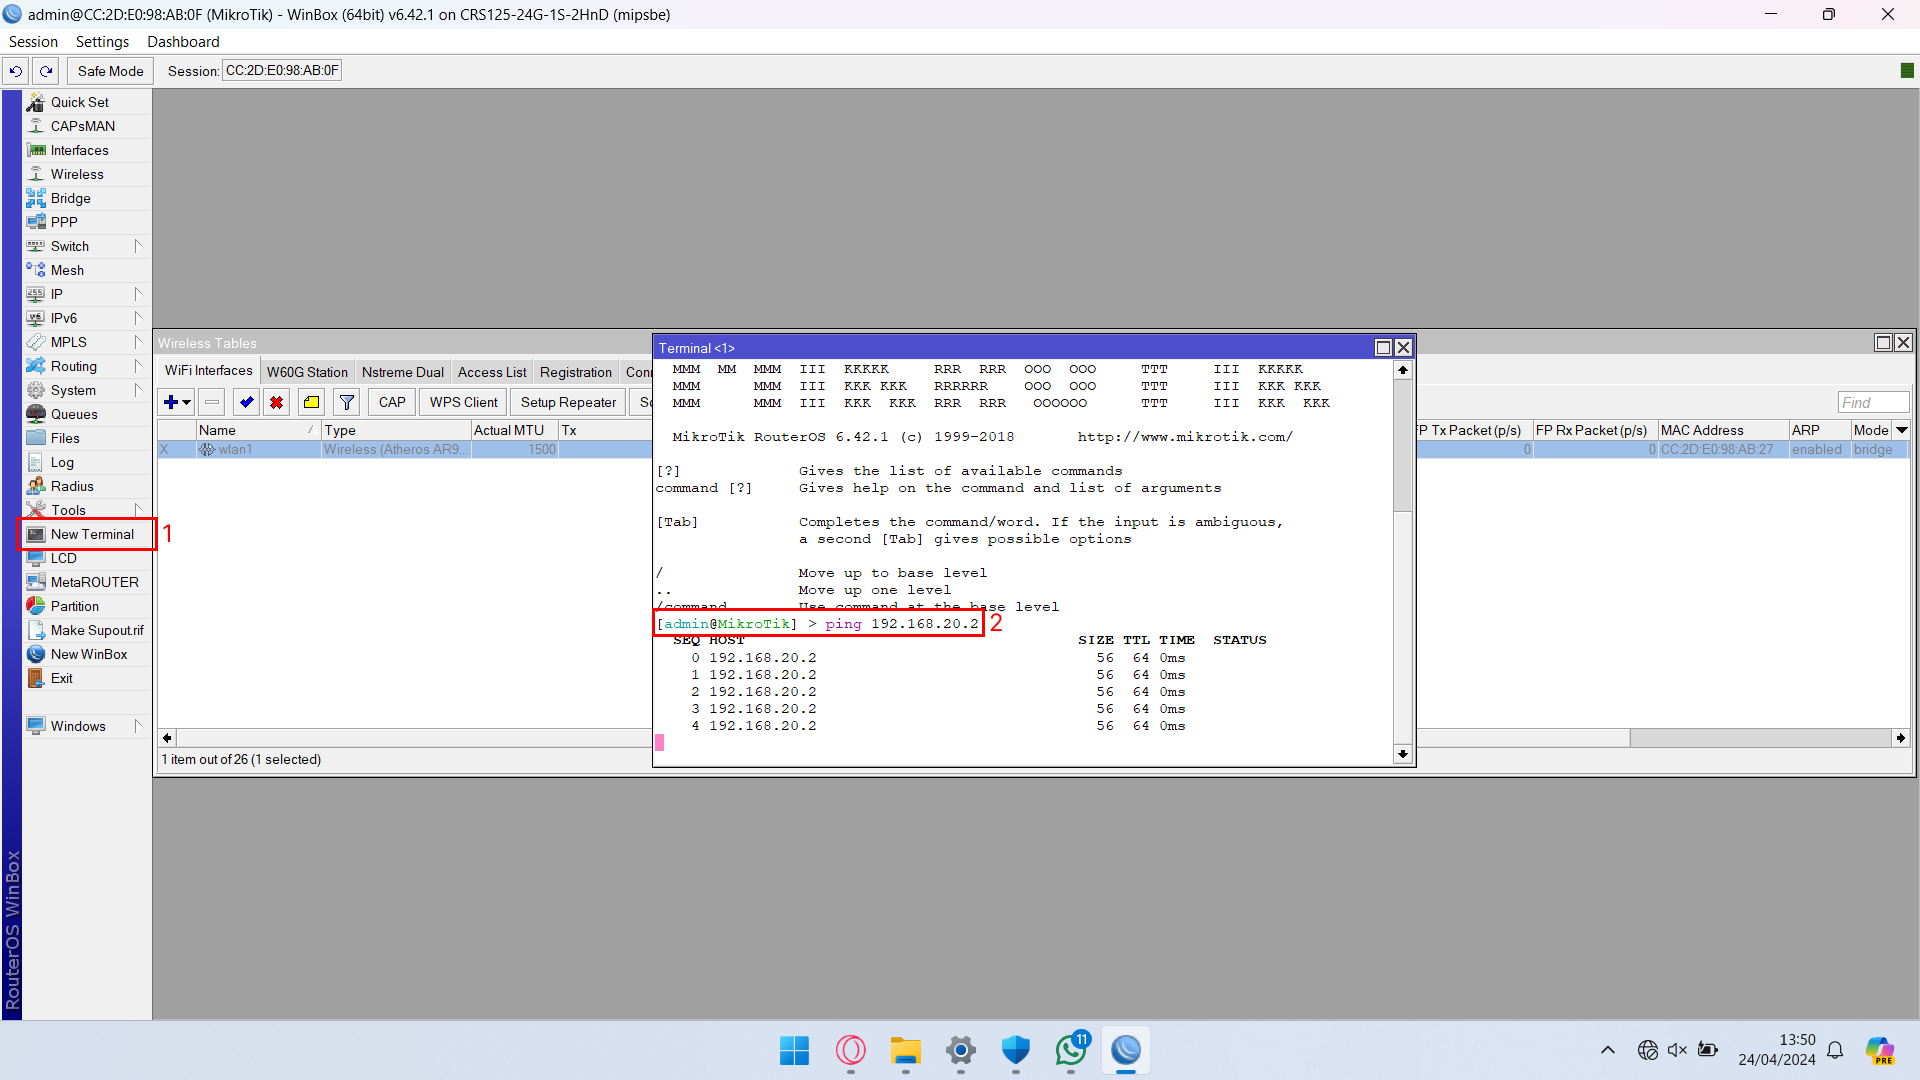
\includegraphics[width=0.9\linewidth]{P2/img/per1/pc1/Step 4.png}
			\caption{Step 1}
			\label{fig:Ping Step 1(Per.1 PC1)}
		\end{figure}
		\item Lakukan tes ping ke Router 1 melalui Router 2
		\begin{figure}[H]
			\centering
			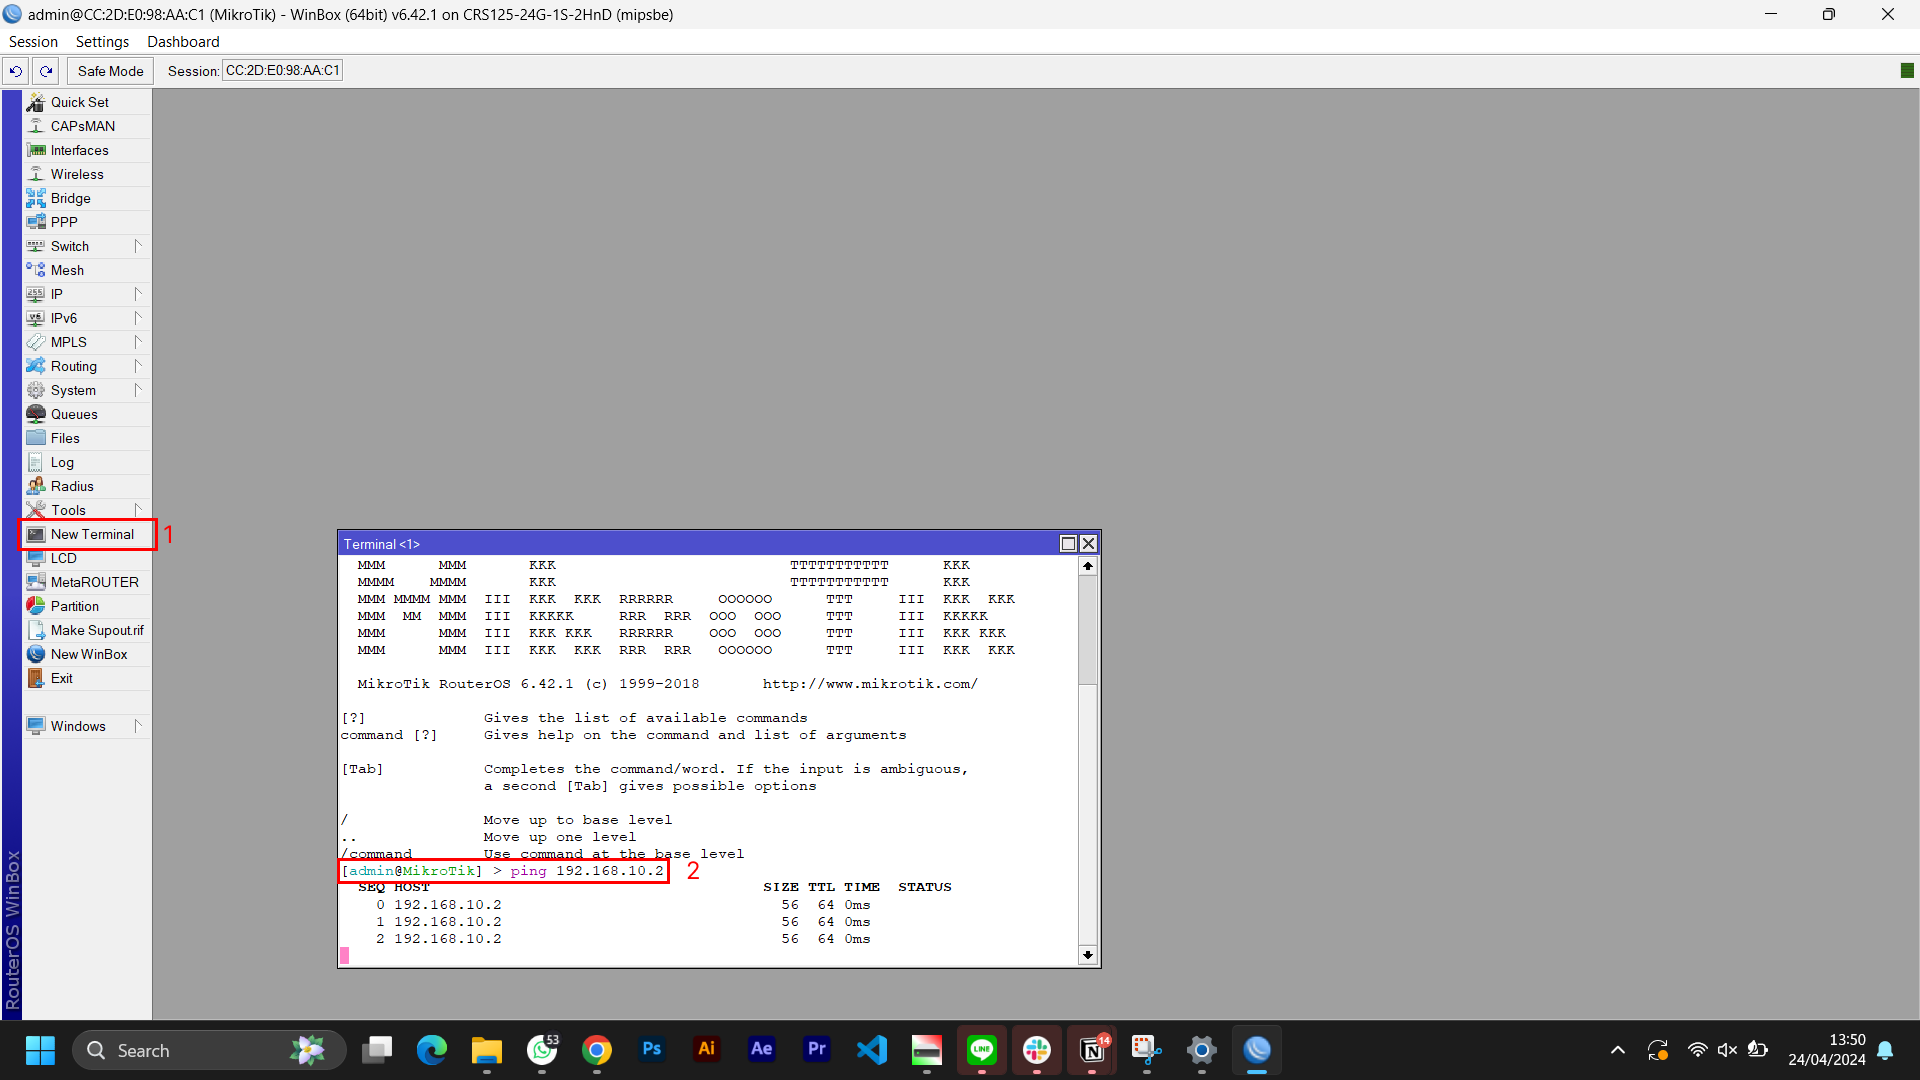
\includegraphics[width=0.9\linewidth]{P2/img/per1/pc2/Step 4.png}
			\caption{Step 2}
			\label{fig:Ping Step 2(Per.1 PC2)}
		\end{figure}
	\end{enumerate}
\end{center}

%======================PERCOBAAN 2==========================%
\subsection{Routing Dinamis}
Pada routing dinamis, terdapat setidaknya 3 jenis, yaitu
\begin{enumerate}
	\item Routing Information Protocol (RIP) RIP adalah salah satu protokol routing dinamis yang menggunakan metrik hop count (jumlah hop) untuk menentukan jalur terbaik. Metrik hop count mengukur jarak antara router pengirim dengan tujuan dalam jumlah hop (melalui berapa banyak router).
	\item Open Shortest Path First (OSPF) OSPF adalah protokol routing dinamis yang menggunakan algoritma Dijkstra untuk menentukan jalur terpendek. OSPF mengumpulkan informasi topologi dari semua router dalam jaringan dan menghitung jalur terbaik berdasarkan bobot (cost) setiap link.
	\item Border Gateway Protocol (BGP) BGP adalah protokol routing eksternal yang digunakan di Internet. BGP memungkinkan router di AS (Autonomous System) yang berbeda untuk berkomunikasi dan menukar informasi routing.
\end{enumerate}

\begin{center}
	\textbf{Konfigurasi Router 1}
	\begin{enumerate}
		\item Buka WinBox dan lakukan koneksi ke Router 1
		\item Berikan IP address pada interface ether2 dan ether 4 yang dapat dibuat pada tab IP > Addresses. Berikan IP address sesuai dengan cara pengaturan IP address yang benar Berikan IP address yang berbeda dengan contoh di modul.
		\begin{figure}[H]
			\centering
			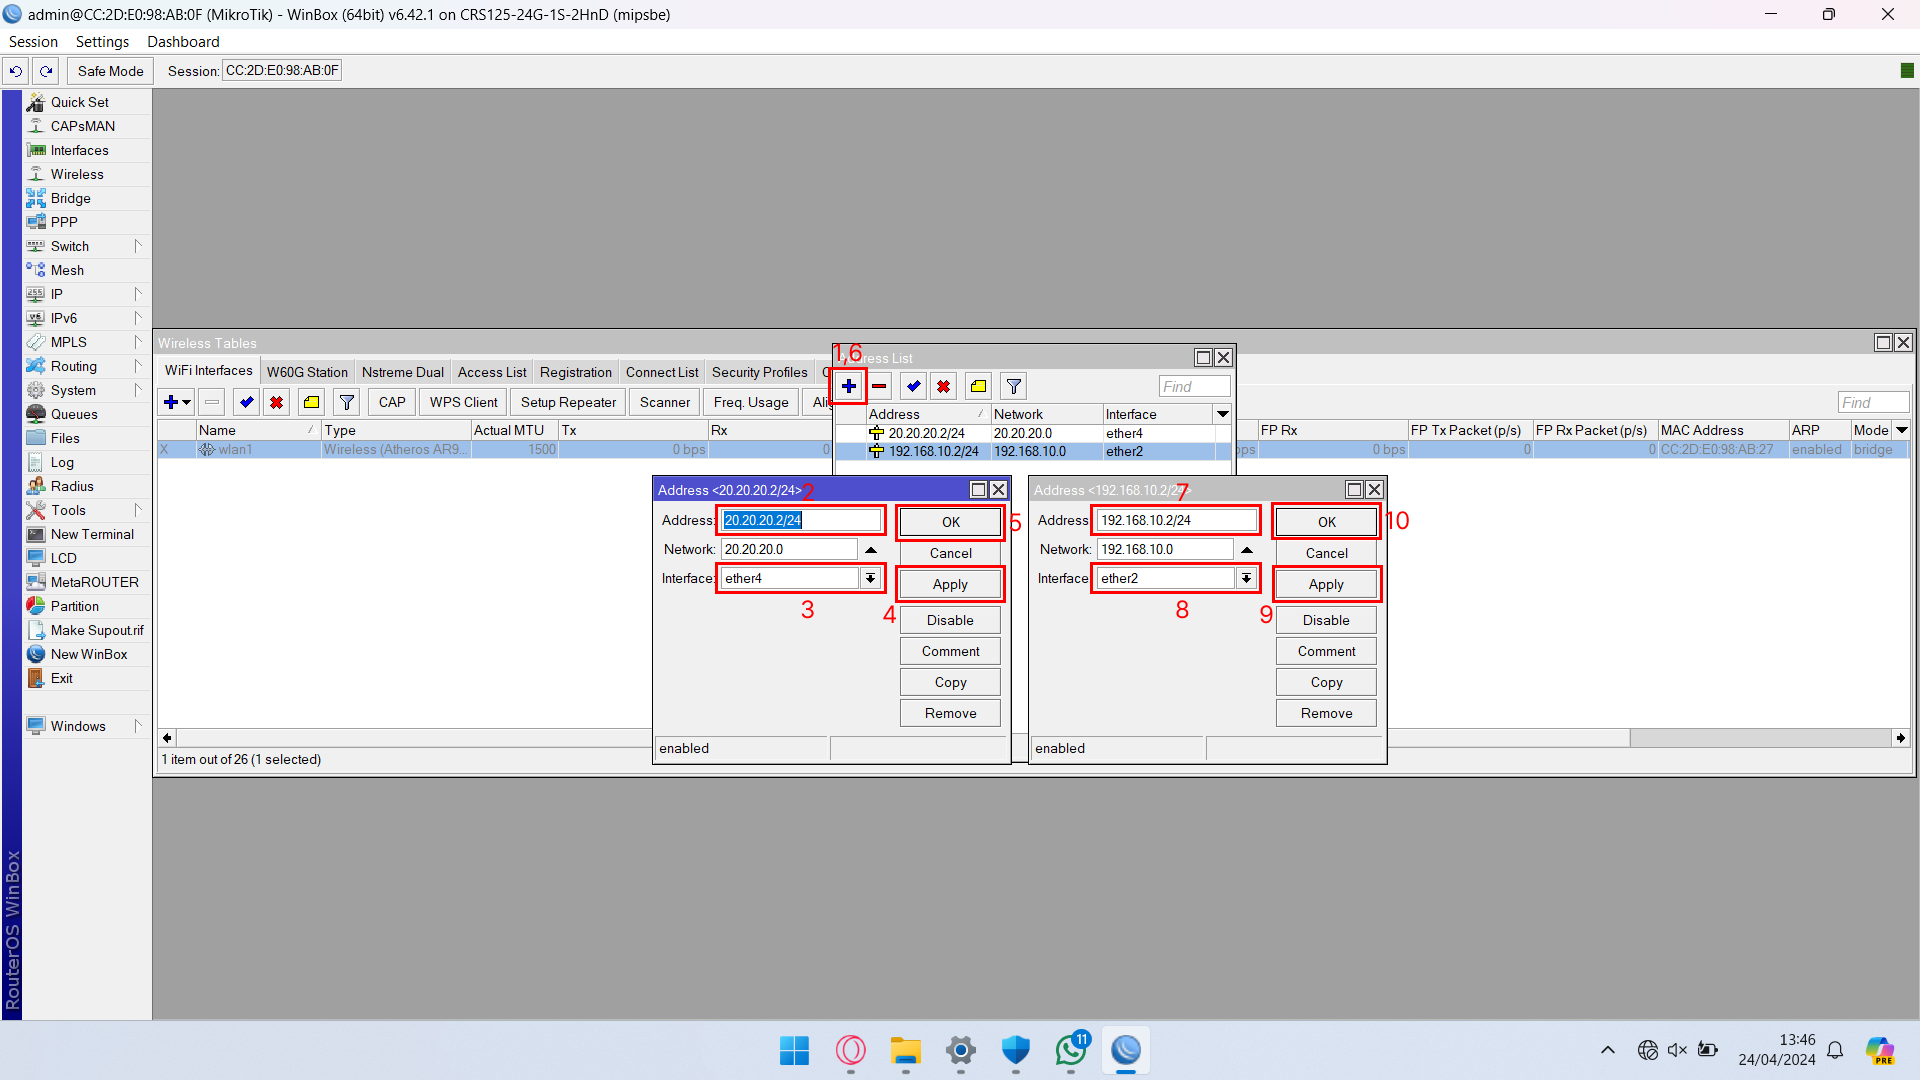
\includegraphics[width=0.9\linewidth]{P2/img/per1/pc1/Step 2.png}
			\caption{Step 2}
			\label{fig:Step 2(Per.2 PC1)}
		\end{figure}
		\item Pada PC 1, lakukan routing dinamis. Buka tab Routing > RIP. 
		\begin{figure}[H]
			\centering
			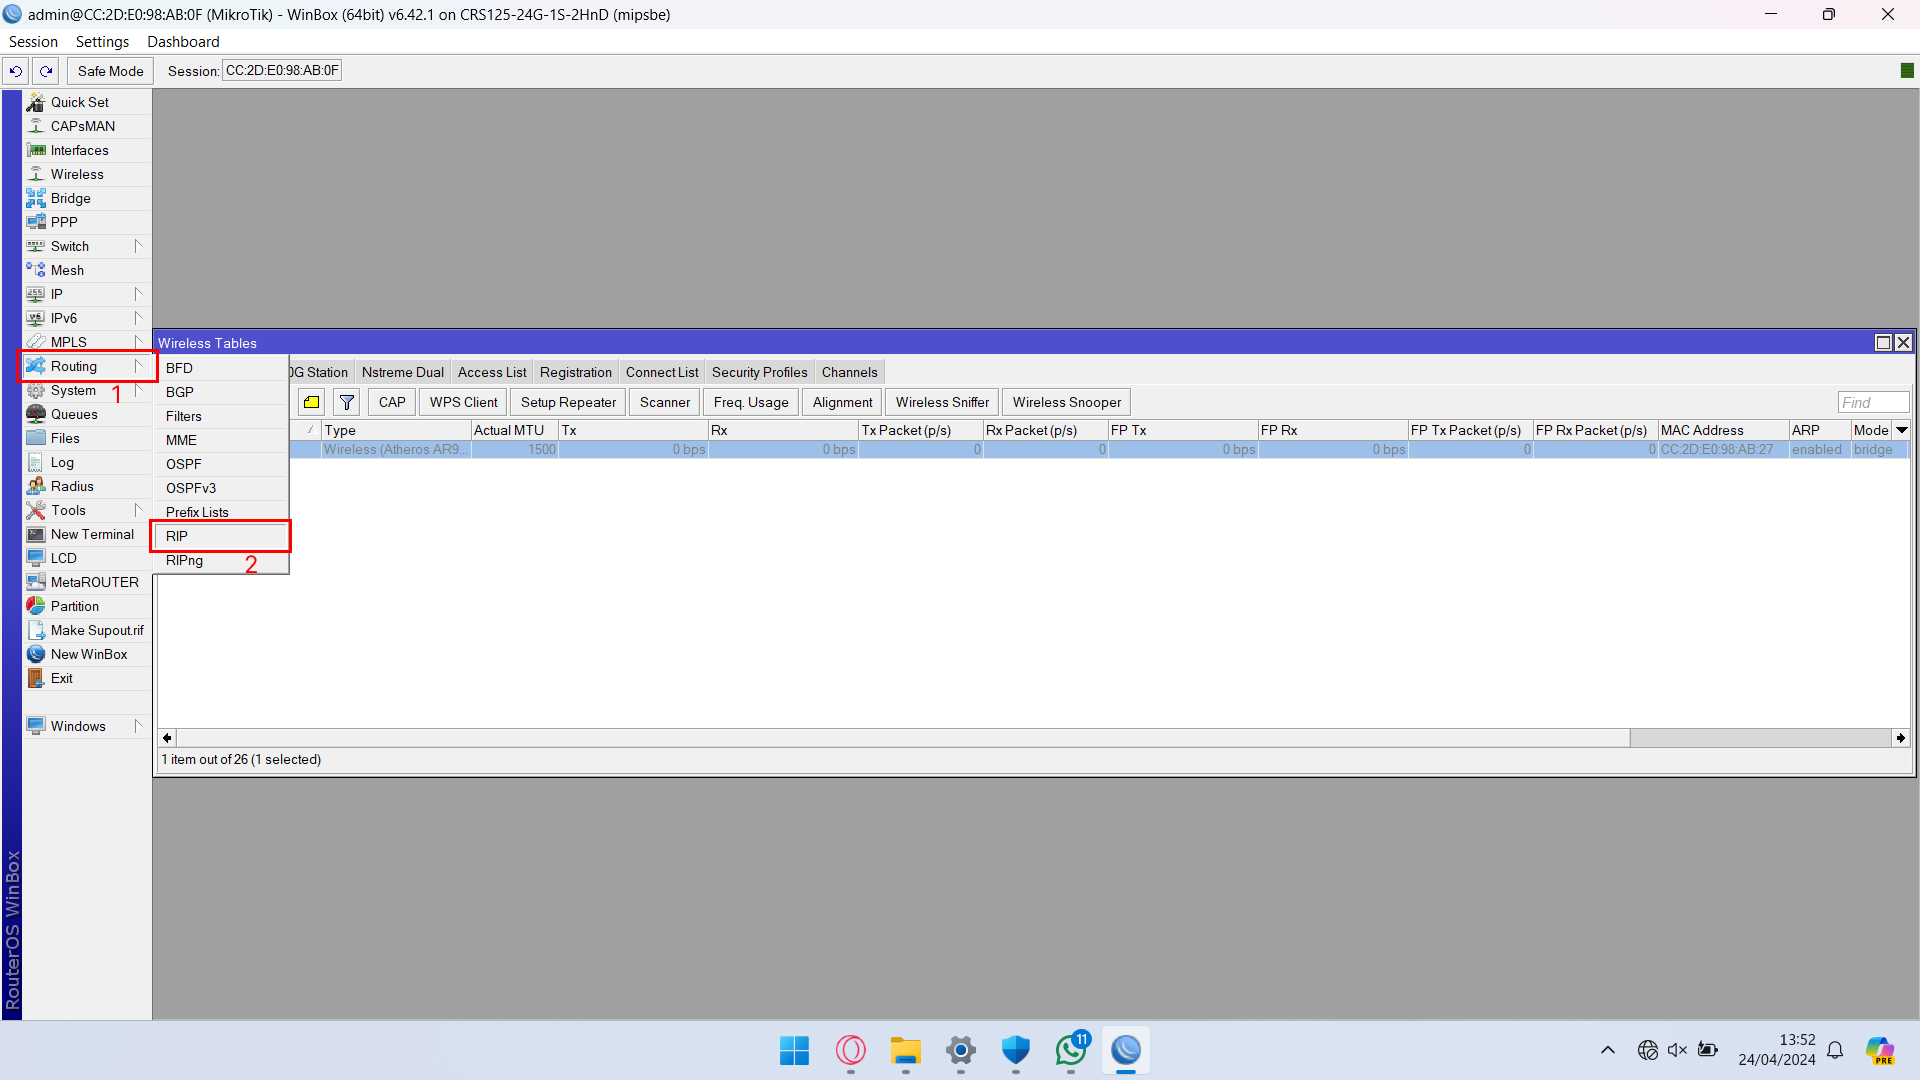
\includegraphics[width=0.9\linewidth]{P2/img/per2/pc1/Step 3.1.png}
			\caption{Step 3.1}
			\label{fig:Step 3.1(Per.2 PC1)}
		\end{figure}
		Pada interface tambahkan interface baru kemudian ubah interface menjadi ether 4 dengan Receive dan Send pada v1.
		\begin{figure}[H]
			\centering
			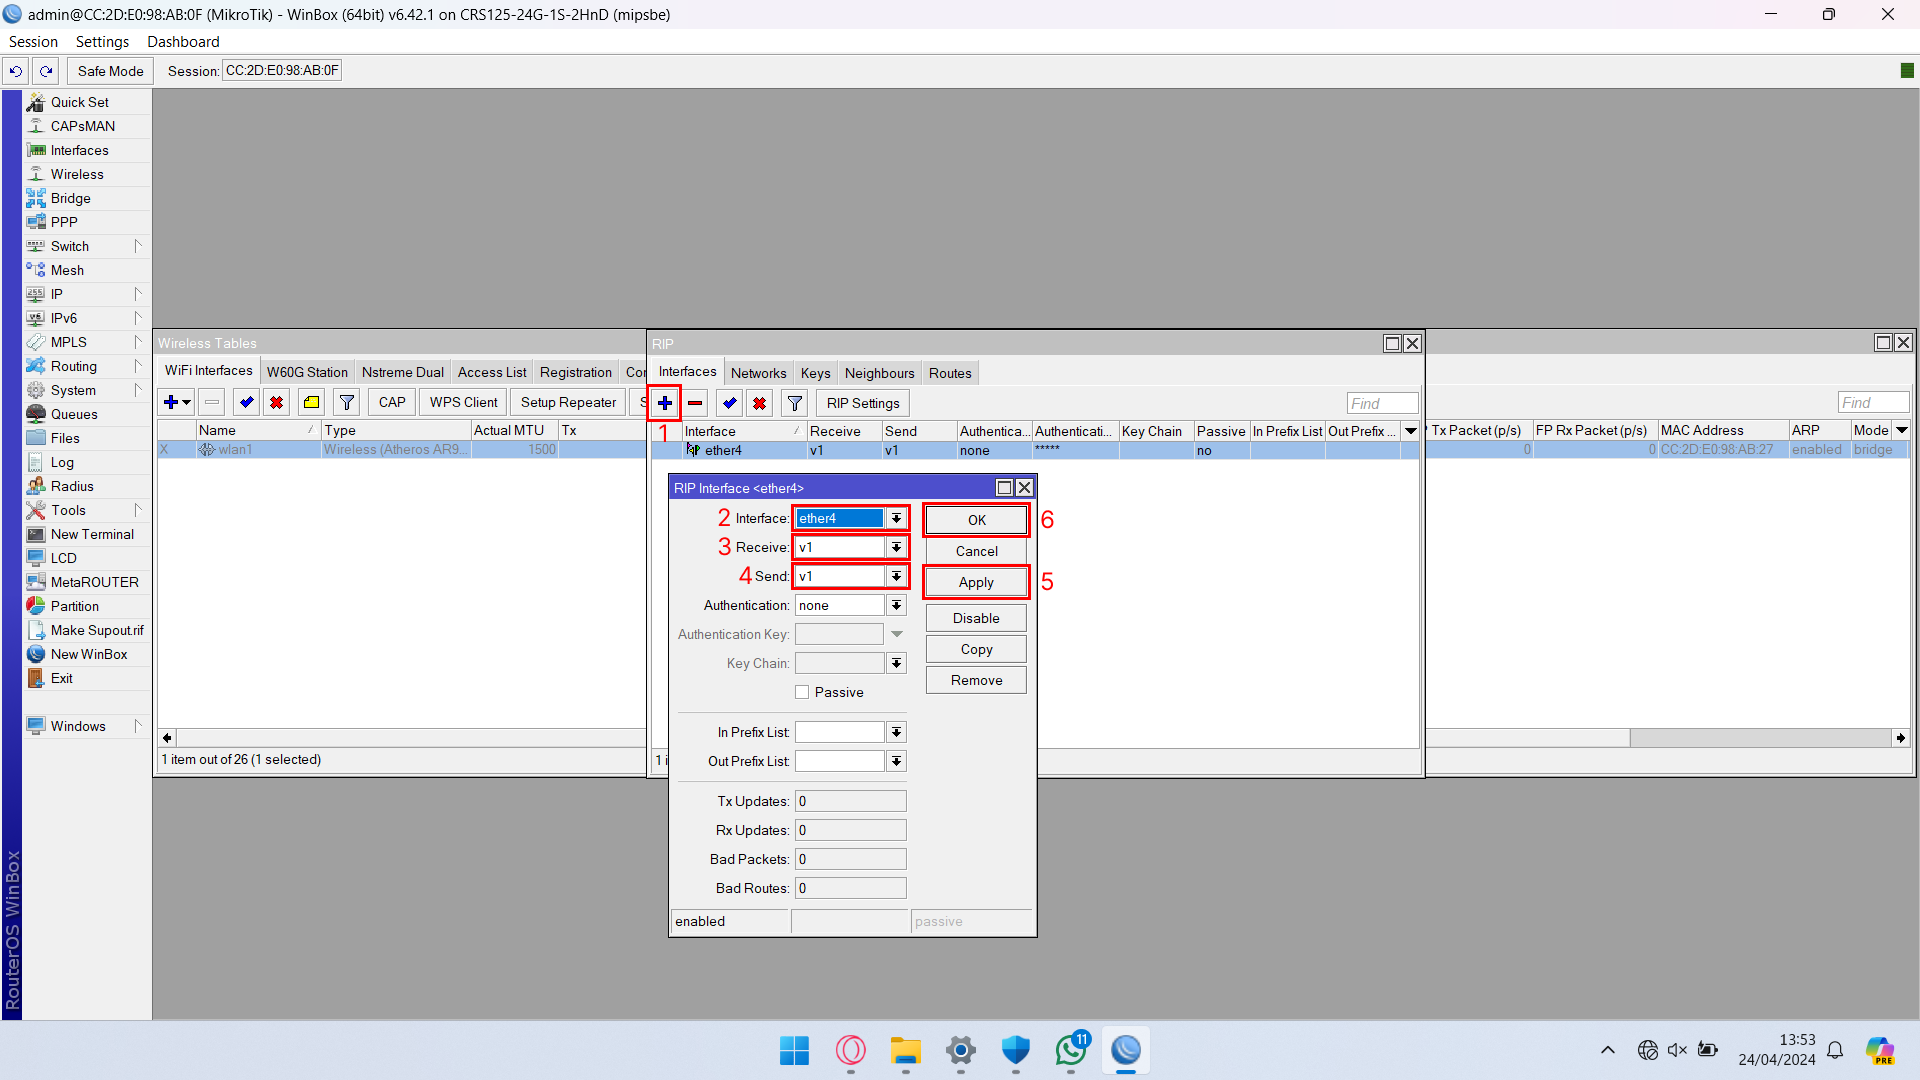
\includegraphics[width=0.9\linewidth]{P2/img/per2/pc1/Step 3.2.png}
			\caption{Step 3.2}
			\label{fig:Step 3.2(Per.2 PC1)}
		\end{figure}
		\item Pada tab Network, tambahkan 2 network baru, yaitu network yang antara PC1 dengan Router 1 dan network antara Router 1 dan Router 2.
		\begin{figure}[H]
			\centering
			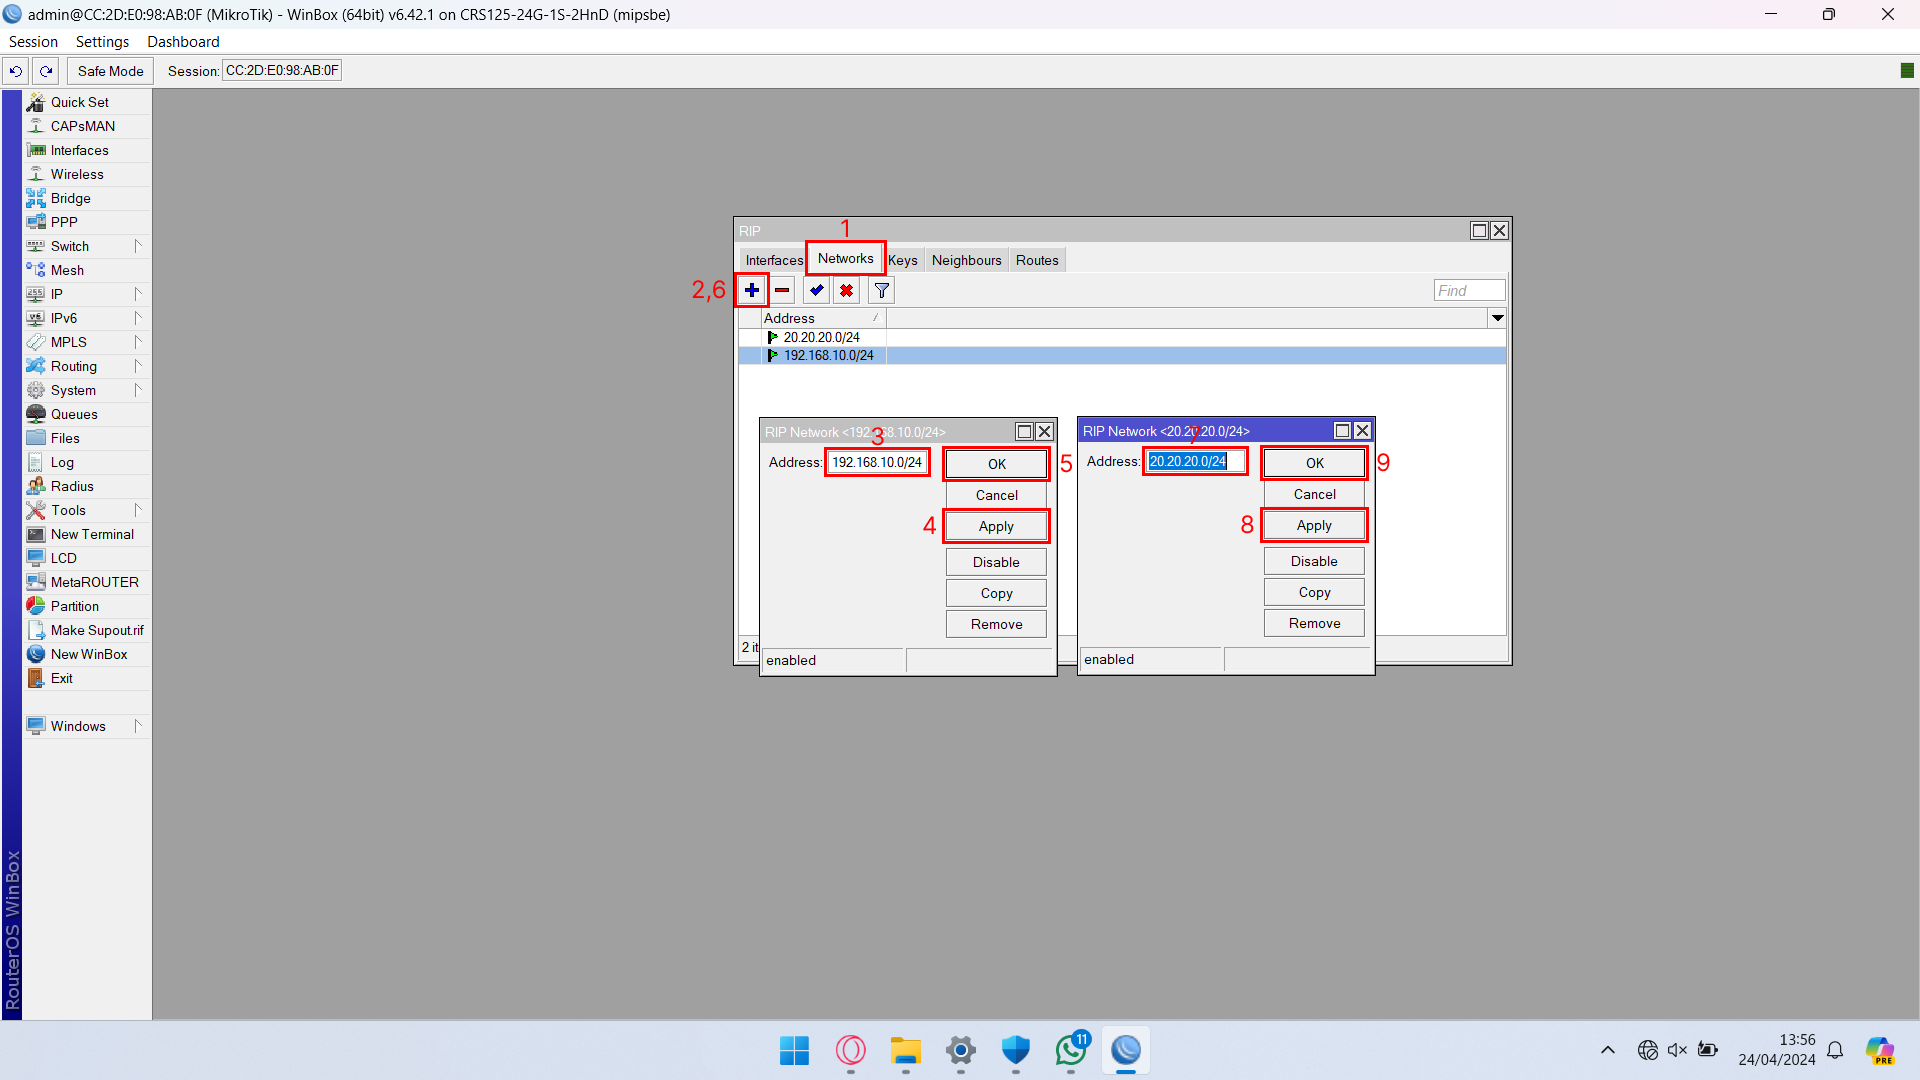
\includegraphics[width=0.9\linewidth]{P2/img/per2/pc1/Step 4.png}
			\caption{Step 4}
			\label{fig:Step 4(Per.2 PC1)}
		\end{figure}
		\item Pada tab Neighbours, tambahkan alamat router yang dituju.
		\begin{figure}[H]
			\centering
			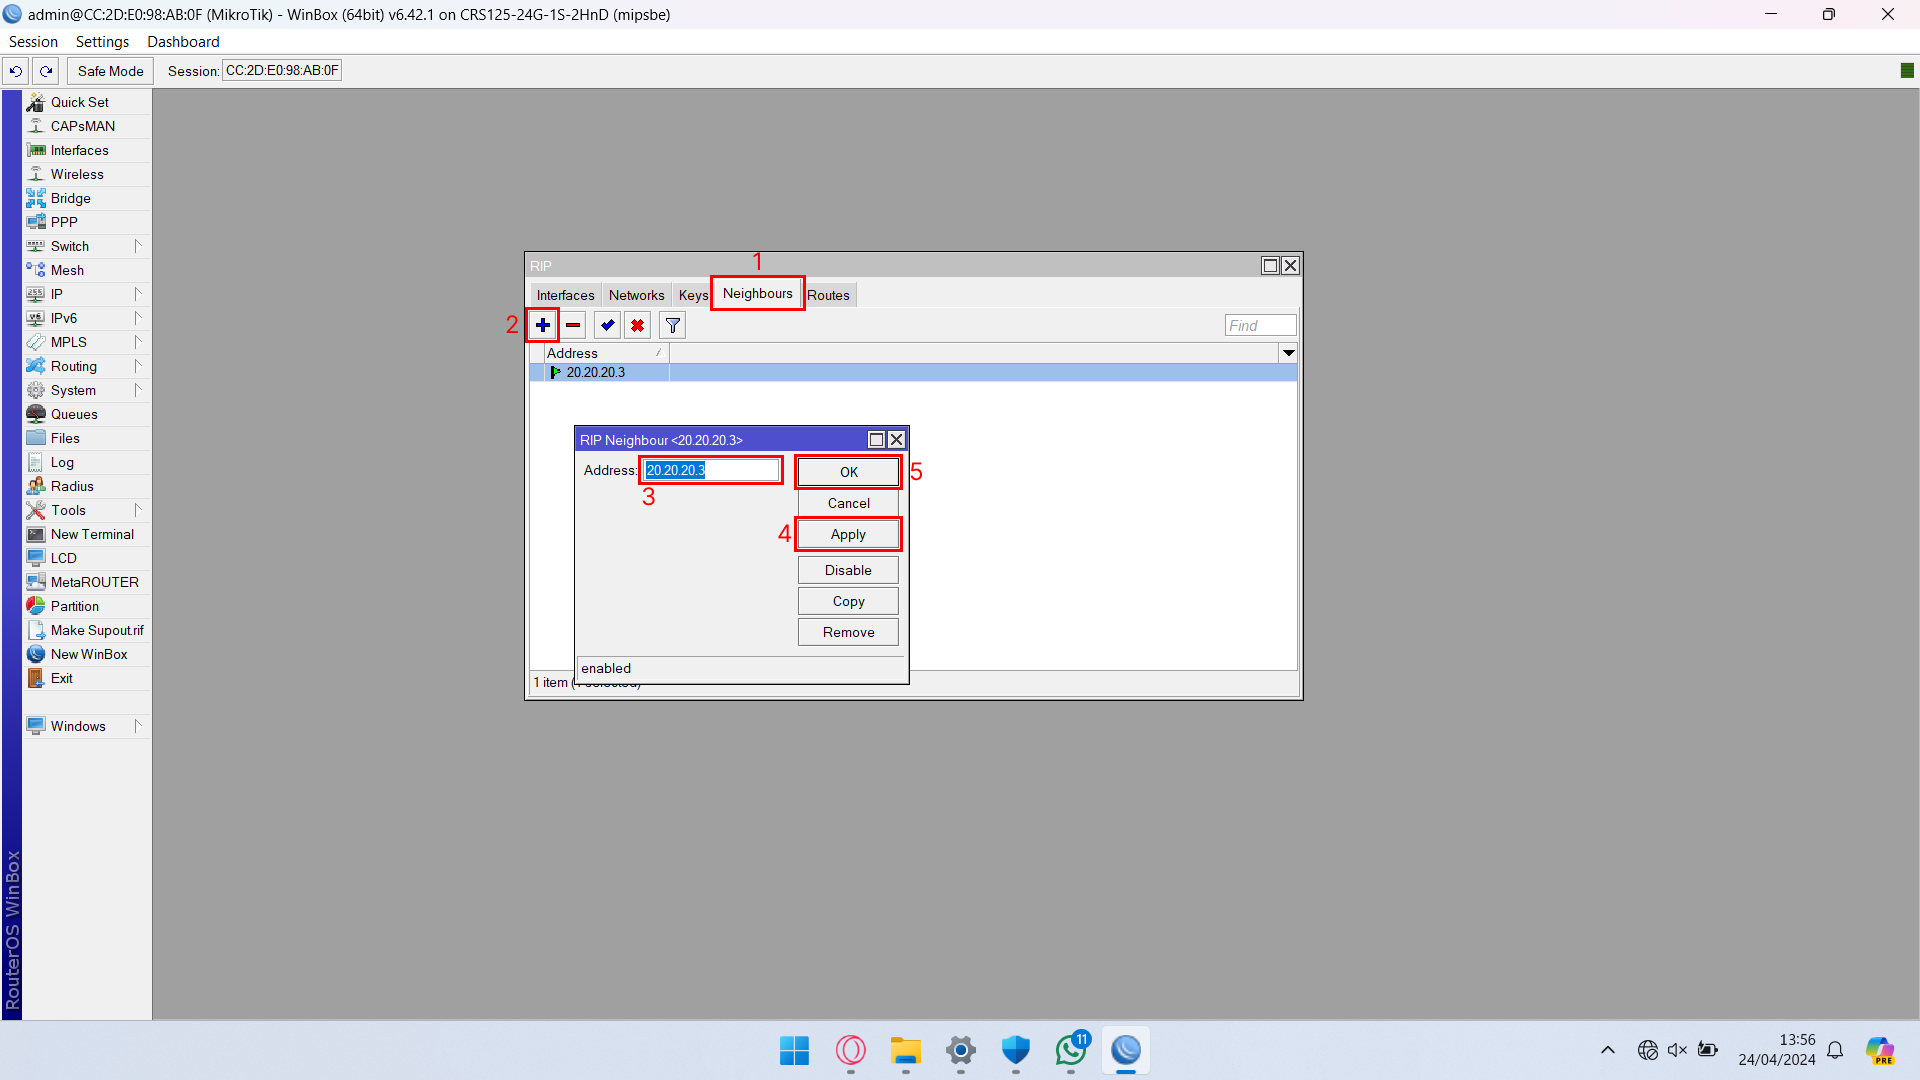
\includegraphics[width=0.9\linewidth]{P2/img/per2/pc1/Step 5.png}
			\caption{Step 5}
			\label{fig:Step 5(Per.2 PC1)}
		\end{figure}
	\end{enumerate}

	\textbf{Konfigurasi Router2}
	\begin{enumerate}
		\item Buka WinBox dan lakukan koneksi ke Router 2
		\item Berikan IP address pada interface ether2 dan ether 4 yang dapat dibuat pada tab IP > Addresses. Berikan IP address sesuai dengan cara pengaturan IP address yang benar. Berikan IP address yang berbeda dengan contoh di modul.
		\begin{figure}[H]
			\centering
			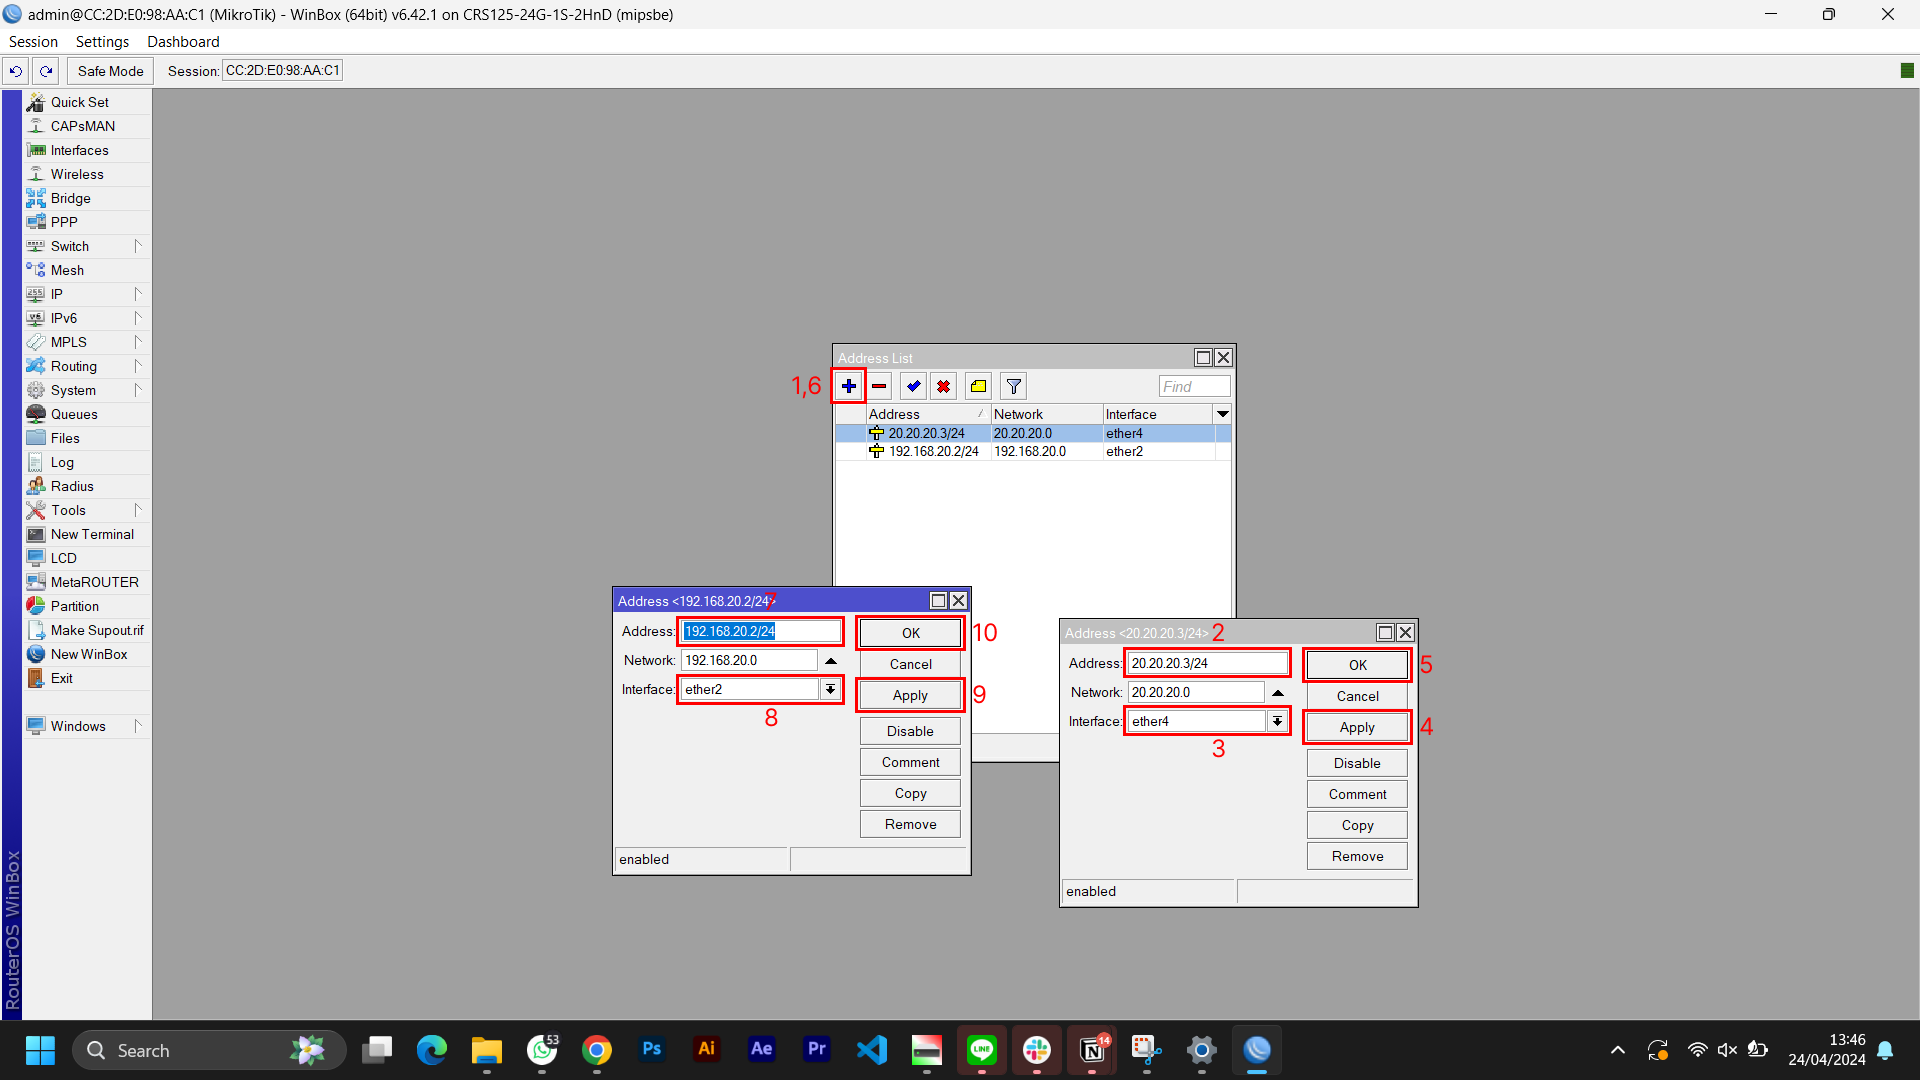
\includegraphics[width=0.9\linewidth]{P2/img/per1/pc2/Step 2.png}
			\caption{Step 2}
			\label{fig:Step 2(Per.2 PC2)}
		\end{figure}
		\item Pada interface tambahkan interface baru kemudian ubah interface menjadi ether 4 dengan Receive dan Send pada v1.
		\begin{figure}[H]
			\centering
			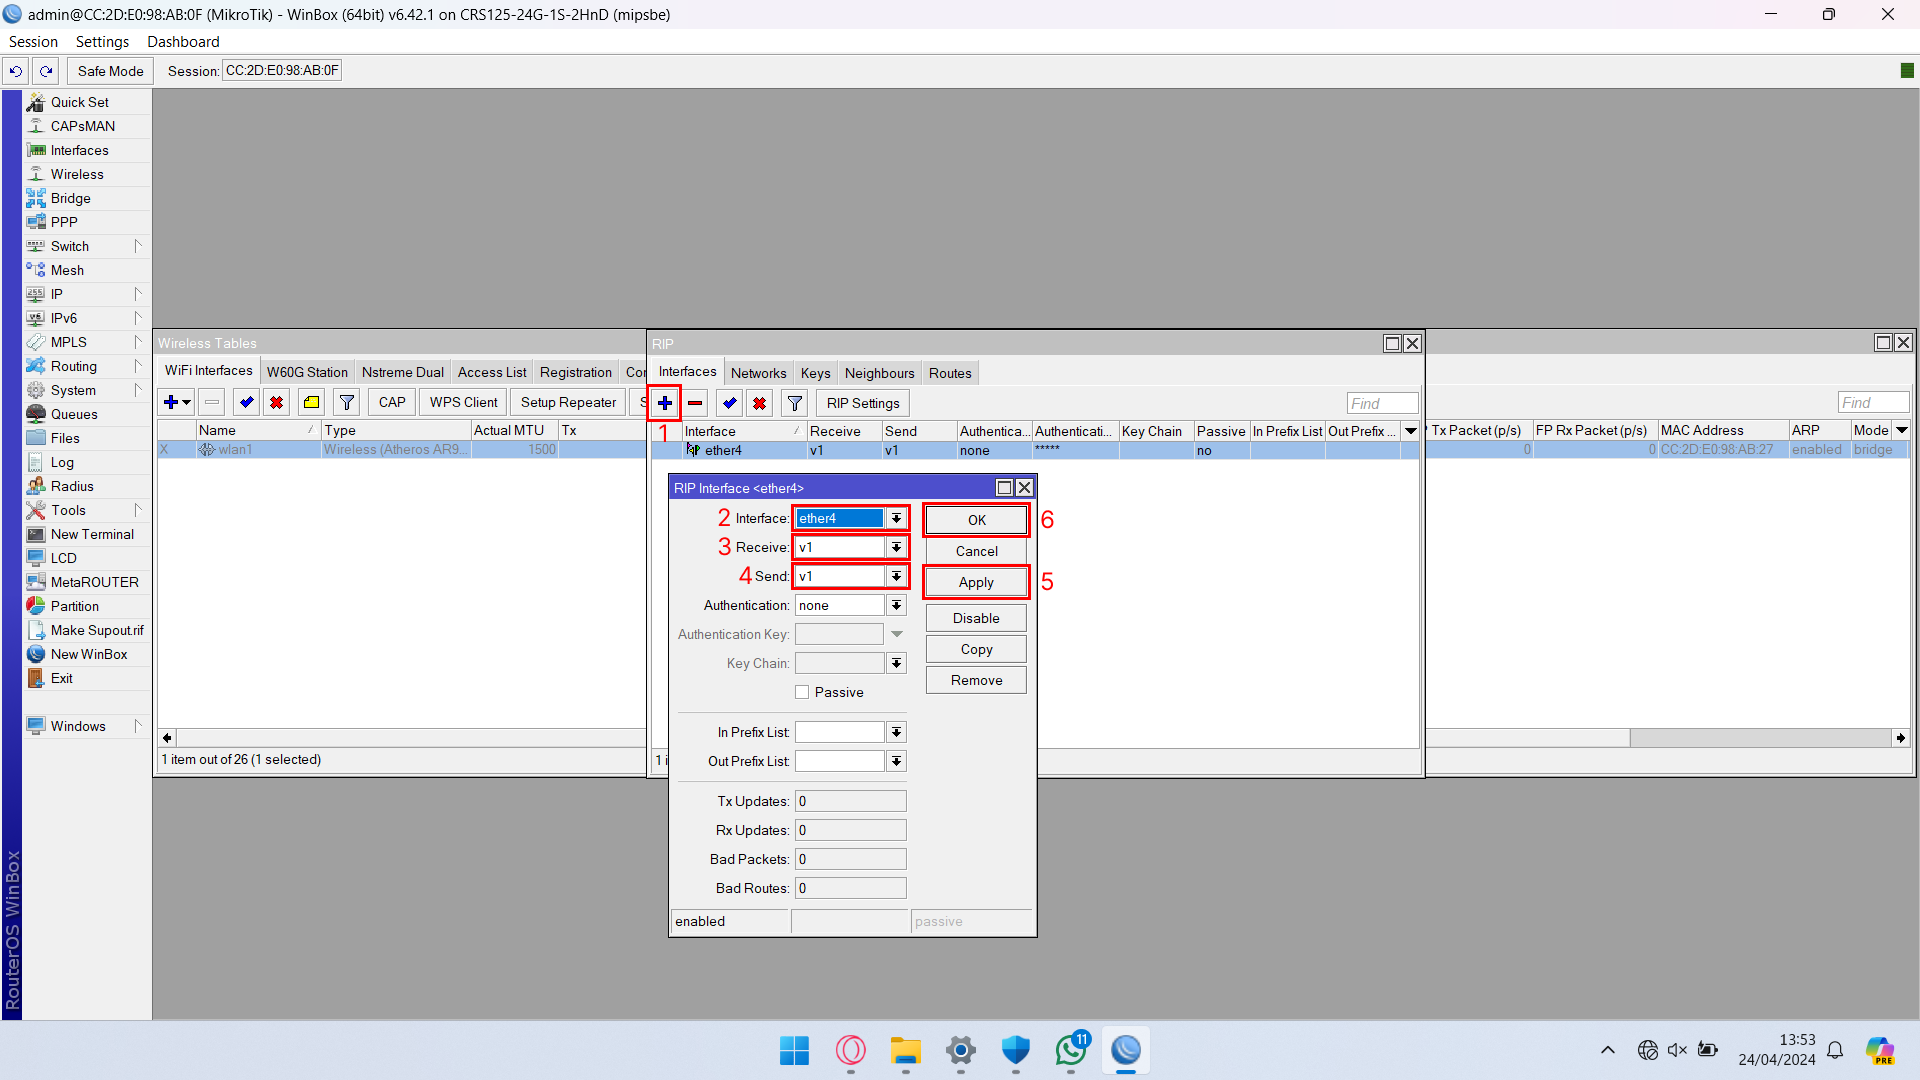
\includegraphics[width=0.9\linewidth]{P2/img/per2/pc1/Step 3.2.png}
			\caption{Step 3.1}
			\label{fig:Step 3.1(Per.2 PC2)}
		\end{figure}
		\item Pada tab Network, tambahkan 2 network baru, yaitu network yang antara PC2 dengan Router 2 dan network antara Router 1 dan Router 2.
		\begin{figure}[H]
			\centering
			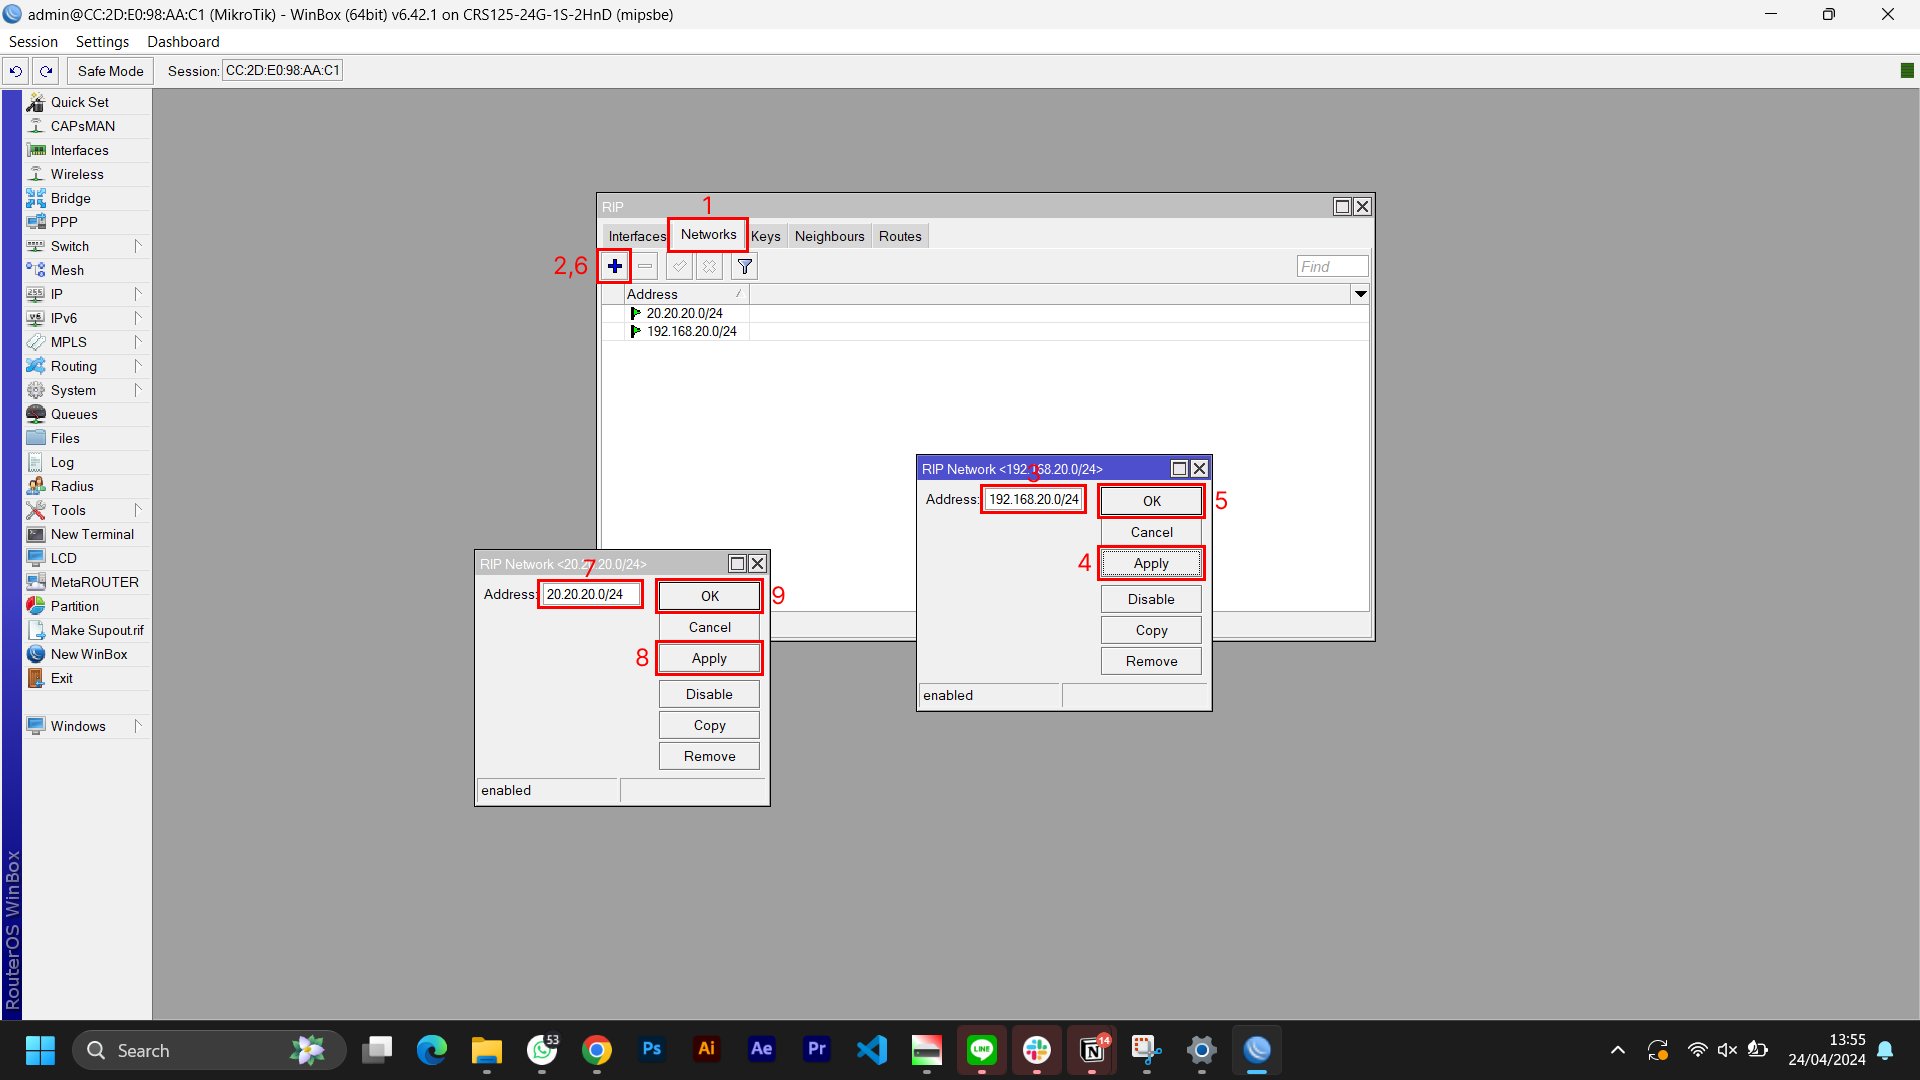
\includegraphics[width=0.9\linewidth]{P2/img/per2/pc2/Step 4.png}
			\caption{Step 3.2}
			\label{fig:Step 3.2(Per.2 PC2)}
		\end{figure}
		\item Pada tab Neighbours, tambahkan alamat router yang dituju.
		\begin{figure}[H]
			\centering
			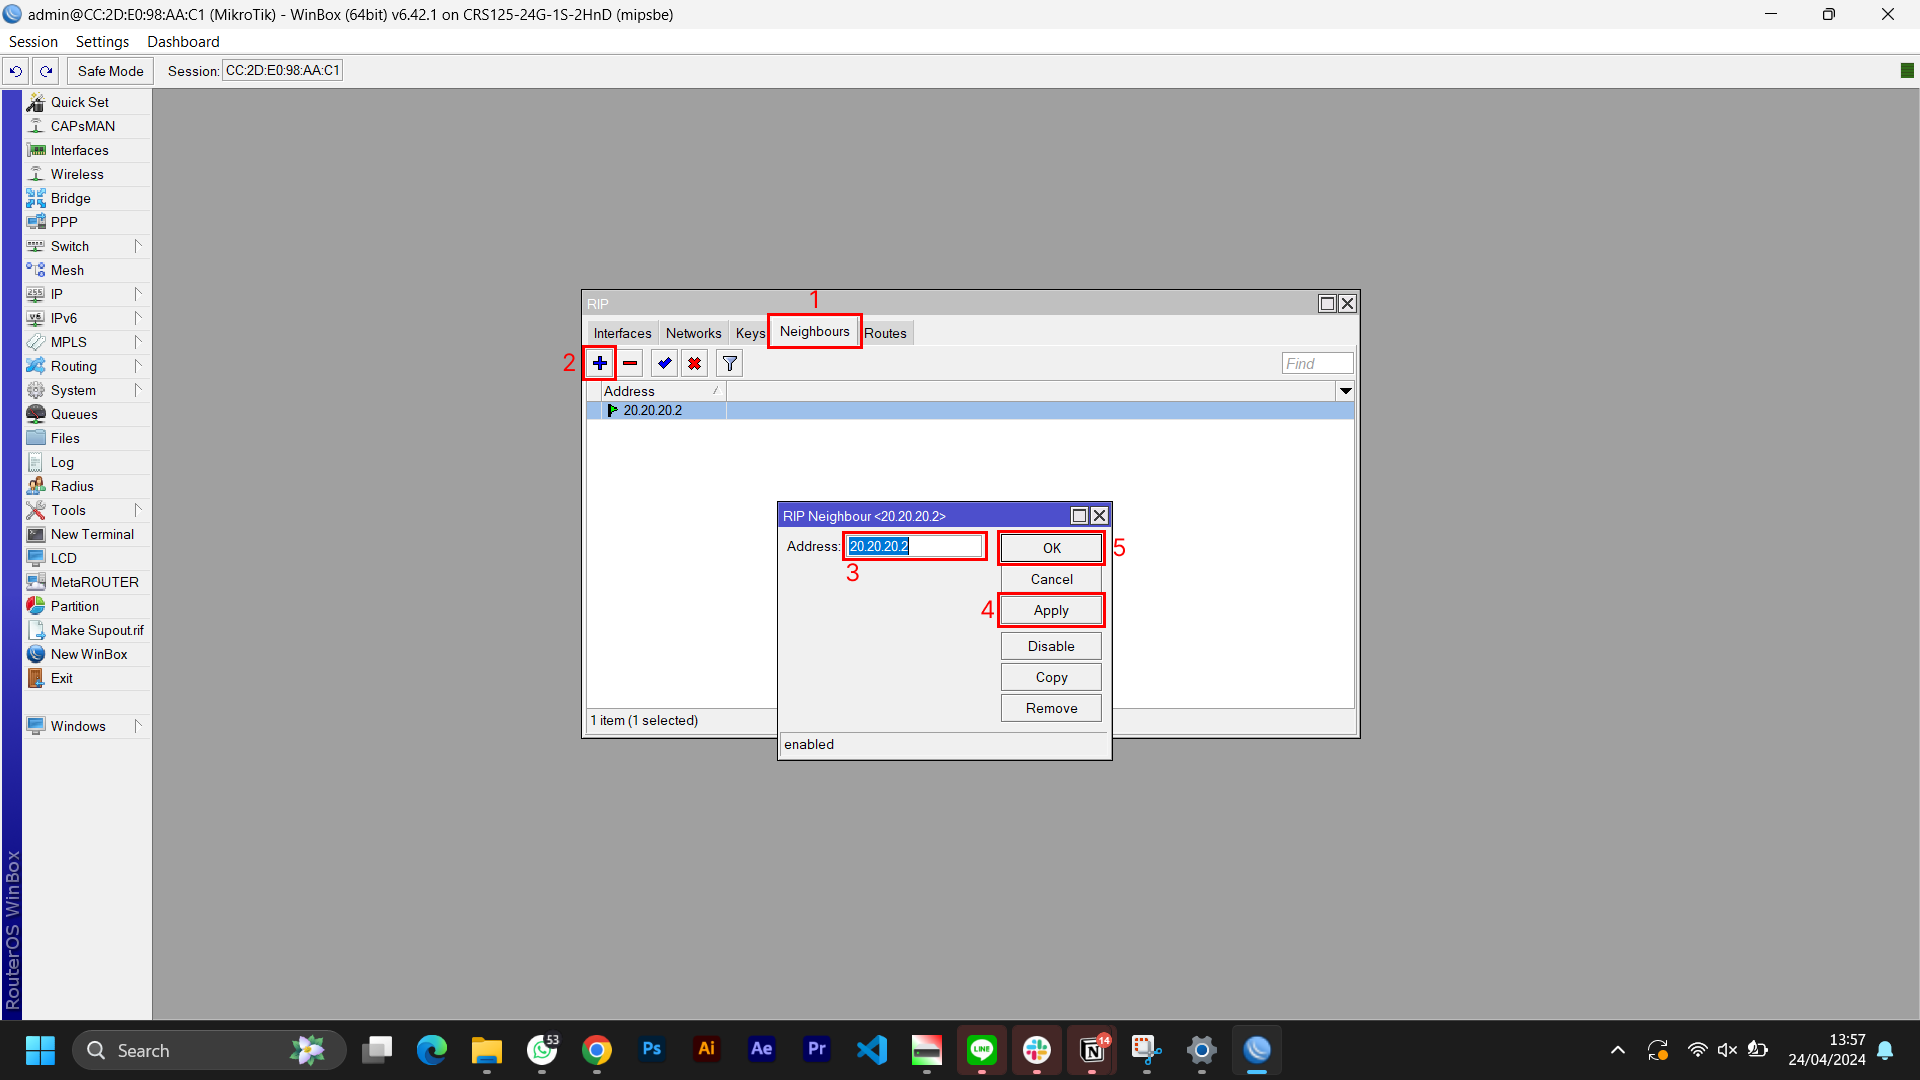
\includegraphics[width=0.9\linewidth]{P2/img/per2/pc2/Step 5.png}
			\caption{Step 4}
			\label{fig:Step 4(Per.2 PC2)}
		\end{figure}
	\end{enumerate}

	\textbf{Pengujian Konfigurasi}
	\begin{enumerate}
		\item Lakukan tes ping dari Router 2 ke Router 1
		\begin{figure}[H]
			\centering
			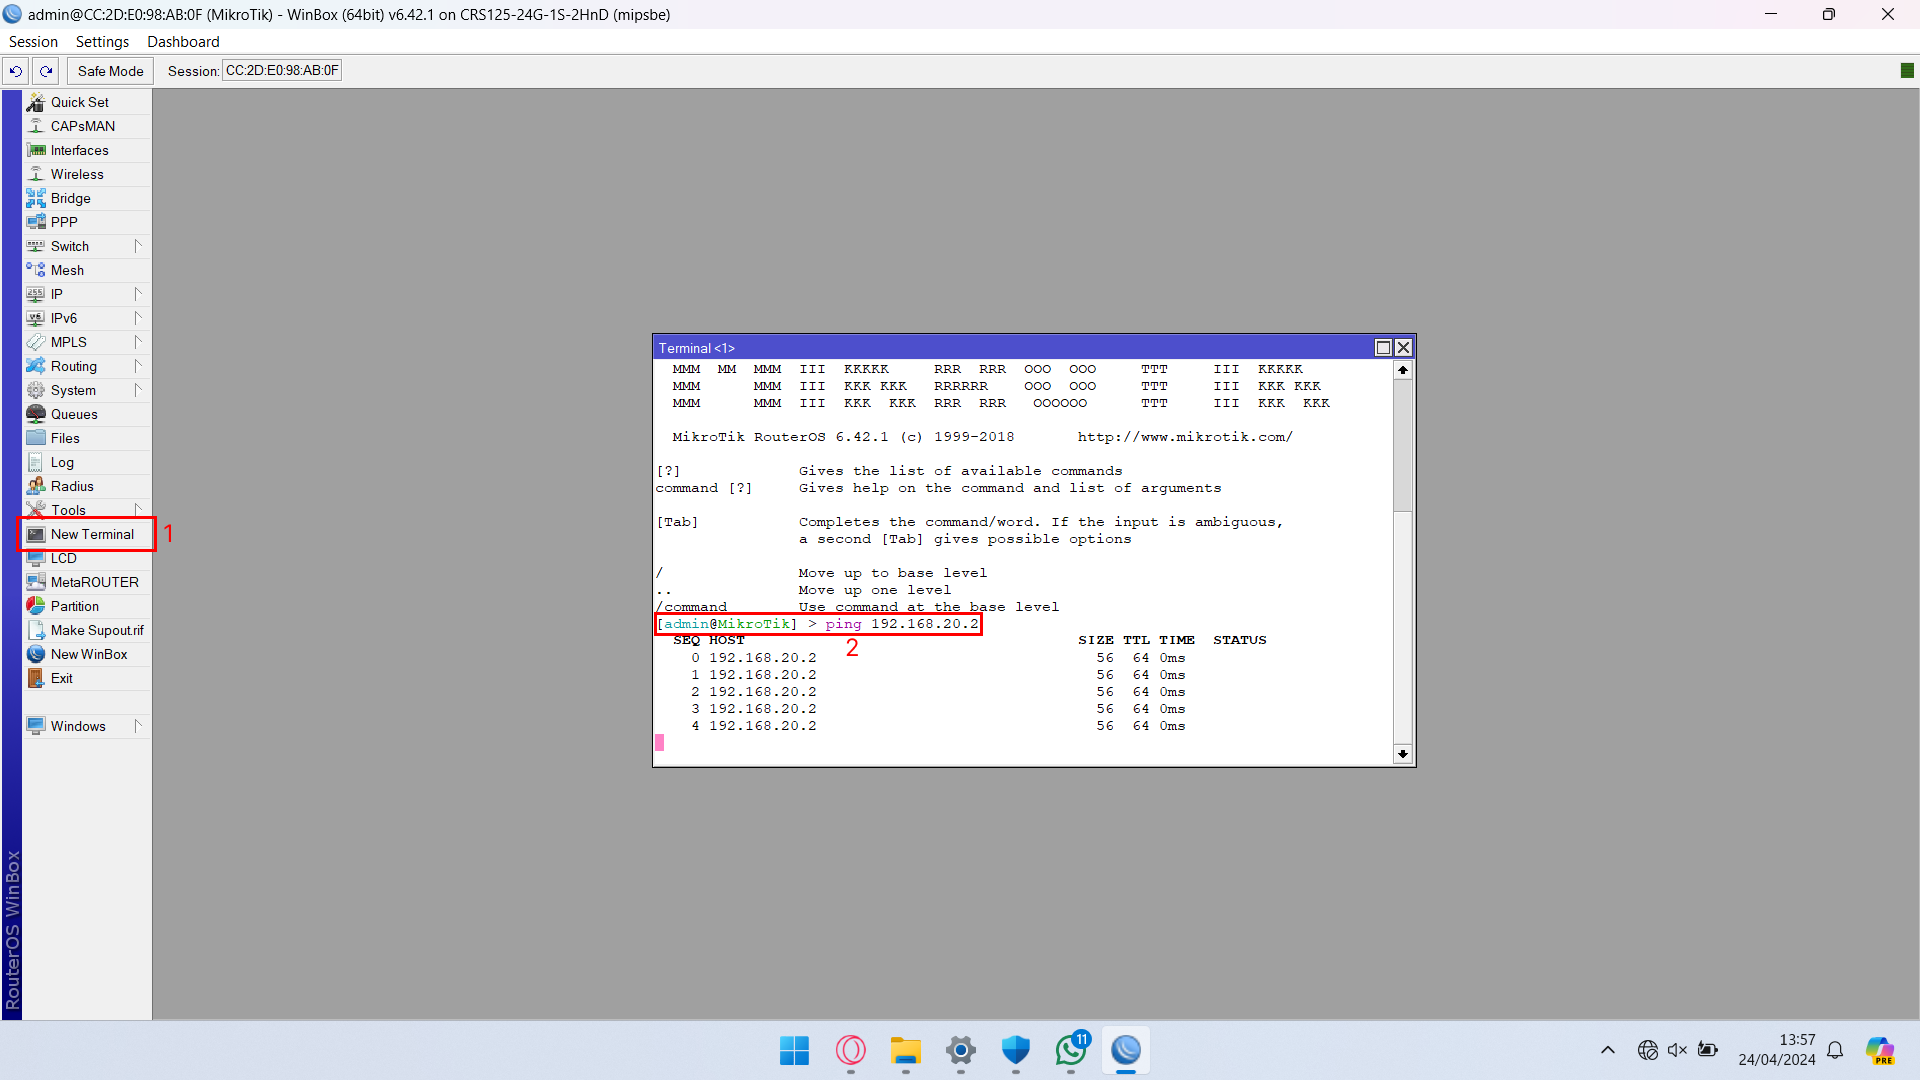
\includegraphics[width=0.9\linewidth]{P2/img/per2/pc1/Step 6.png}
			\caption{Step 1}
			\label{fig:Ping Step 1(Per.2 PC1)}
		\end{figure}
		\item Lakukan tes ping dari Router 1 ke Router 2
		\begin{figure}[H]
			\centering
			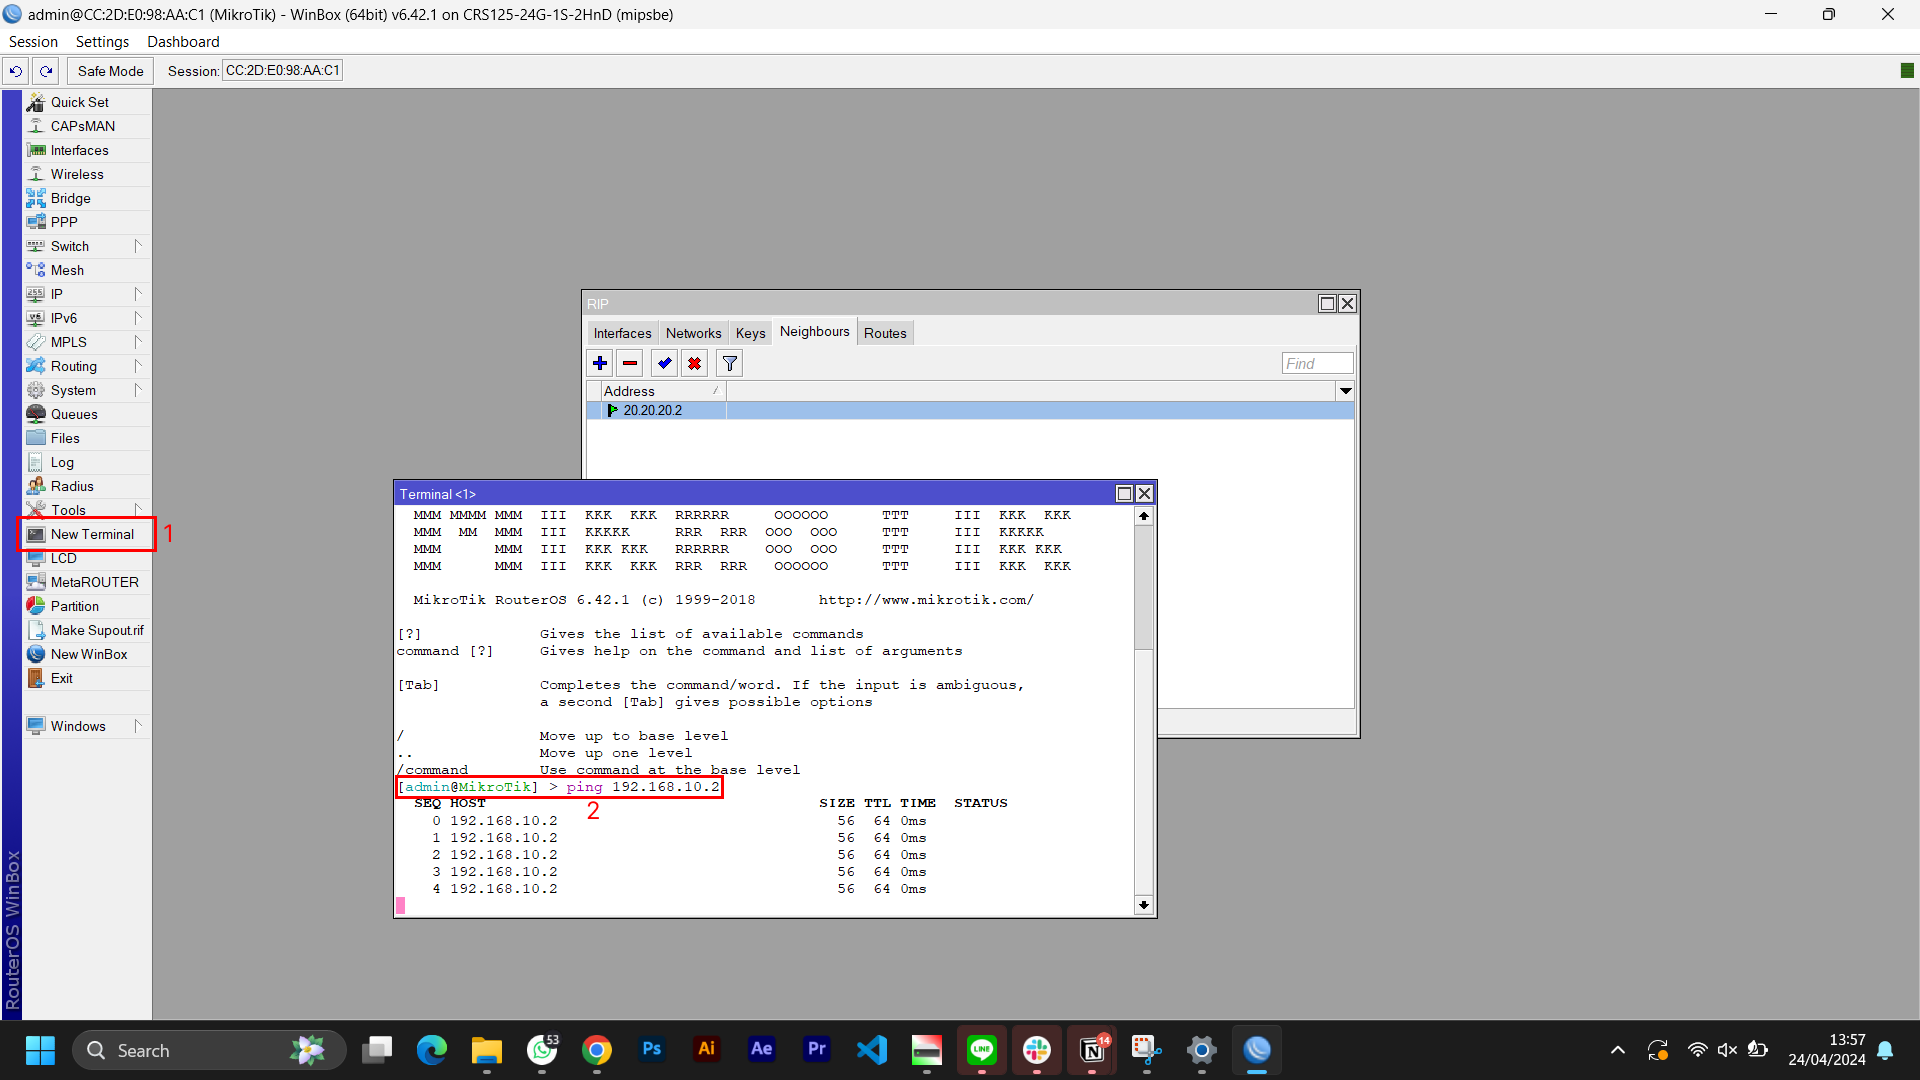
\includegraphics[width=0.9\linewidth]{P2/img/per2/pc2/Step 6.png}
			\caption{Step 2}
			\label{fig:Ping Step 2(Per.2 PC2)}
		\end{figure}
	\end{enumerate}
\end{center}

%===========================================================%
\section{Hasil yang didapat}
Memahami dan mengkonfigurasi routing dinamis RIP dengan tepat.

%===========================================================%
\section{Kesimpulan}
Dalam mengkonfigurasi routing RIP, diperlukan pemahaman dasar mengenai setting IP Address dan Subnetting, dan juga diperlukan ketelitian dan fokus agar berhasil


